\documentclass[11pt]{report}
\usepackage{epsfig}
\usepackage{url}
\usepackage{pslatex}
\usepackage{fullpage}
\usepackage{moreverb}
\usepackage{supertabular}

\newcommand{\HRule}{\rule{\linewidth}{0.5mm}}

\oddsidemargin -7mm 
\textheight 9.0in
\textwidth 15.3cm \setcounter{secnumdepth}{4}
\setcounter{tocdepth}{4} \pagestyle{myheadings}

\def \baselinestretch{1,2}

\usepackage{calc}
\newlength{\topspace}
\setlength{\topspace}{0in}

%turn on 1.5 line spacing
\renewcommand{\baselinestretch}{1.5}

\begin{document}


\begin{titlepage}
{\sffamily
	\begin{minipage}{0.3 \columnwidth}
	\psfig{figure=images/crest.ps,width=1.2in}
	\end{minipage}
	\begin{minipage}{0.55 \columnwidth}
	\noindent \rule{\linewidth}{0.25mm}
	\begin{center}
	{\Large{Department of Computing Science \\ \ \\ University of Glasgow \\
Lilybank Gardens\\
Glasgow G12 8QQ\\ \ \\
	{\scshape CS4H Project Report \\ Craig Macdonald, 2003/2004}}
	
}
\end{center}
\noindent 
\rule{\linewidth}{0.25mm}
\end{minipage}

\begin{center}
\ \\
\ \\
\ \\
\ \\
\ \\
\ \\
\ \\
{\LARGE  {\bf\sffamily Labrador - a distributed web crawler \\for \\a departmental search engine}

\ \\

by\\

\ \\

{\sffamily Craig Macdonald}\\
{\sffamily macdonch@dcs.gla.ac.uk}

}

\end{center}
}
\end{titlepage}
\pagestyle{myheadings}
\renewcommand{\thepage}{\roman{page}}

\newpage
%\thispagestyle{empty}

\noindent I hereby give my permission for this project to be shown to other
University of Glasgow students and to be distributed in an electronic
format. {\bf Please note that you are under no obligation to sign this
declaration, but doing so would help future students. }

\begin{description}
\item [Craig Macdonald] \ \\  \ \\
\HRule

\end{description}
\addcontentsline{toc}{chapter}{Education Use Consent}

\begin{center}{\bf\Large Abstract}\end{center}
This report describes the development of Labrador, a distributed scalable web crawler, for use with the Terrier web Information Retrieval framework and the development of a basic web frontend to the Terrier system. The issues affecting the development and running of a crawler are discussed, as is the distributed architecture that was developed to provide the scalable framework.\\

{\bf Keywords:} Search, Information Retrieval, Crawler, Spider, Framework, Distributed
\addcontentsline{toc}{chapter}{Abstract}

\newpage
\tableofcontents
\newpage

\setcounter{page}{1}
\renewcommand{\thepage}{\arabic{page}}


\chapter{Introduction}

\section{Preliminaries}
This project is concerned with building a web crawler and integrating it with a pre-existing search framework and building a web frontend to the search framework.
\section{What is a Crawler?}
A crawler, spider or robot\footnotemark is a program designed and written to download, save and follow any links from pages on the Internet. This allows the Information Retrieval providers, commonly known as the search engines, to provide search services on the Internet, as they have already indexed the pages they have downloaded. Without a crawler, a search engine would have to download and index pages in response to each search queries, which is clearly unrealistic given the size of the Internet. \\
\footnotetext{In this report I shall use the word crawler, but the word is interchangeable with spider or robot.}
\ \\
Crawlers are also used by law enforcement organisations to monitor the Internet web pages with criminal elements and many smaller tasks, including some less acceptable uses, such as crawling to obtain email addresses.\\
\ \\
Current generation commercial crawlers, such as that used by Google, do not download every page on the Internet due to the prohibitively large storage requirements and network costs involved. Therefore effort is spent ensuring that the best pages are downloaded earlier, increasing the likelihood of having downloaded the best pages when the crawl is terminated.\\

\section{Difficulties in writing a crawler}
Although fundamentally a simple program, many additional requirements make a scalable high-performance crawler a difficult challenge. Firstly, there are several de-facto protocols that must be observed to ensure that your crawler is seen as polite when crawling a website. The robots.txt and Meta-Robots standards are designed such that crawlers can determine whether the webmaster of that site or page wishes it to be crawled or not. Secondly, crawlers should be polite in their usage of a given host. Overloading any one host will make the owner of the crawler unpopular, which could possibly result in it being banned from connecting to that site again. This is counter-productive, as the content of that site is then unavailable to users of the search engine.To this end, crawlers must leave a gap of seconds between fetches from individial hosts. In Labrador this is known as Host Delay.\\
\ \\
The crawler should be scalable, such that it can maintain a respectable rate of fetches each second in order to cope with the huge size of the web. To fetch billions of documents (the current perceived size of the Internet), the crawler must be able to achieve and maintain fetch rates of several hundred URLs/second. A crawl rate of this magnitude is necessary to ensure that a reasonable Internet crawl of 1 billion documents will be completed in under a month. One month is the normal refresh period for Internet search engines.\\
\ \\
Crawlers also have to beware of crawler traps. Traps are sites which once the crawler starts to crawl, it may never escape, as the site will continue to generate new links. Some traps are intentional, say perhaps to trap impolite robots, or email address crawlers (for spamming purposes). Unintentional traps are mostly web frontends to large databases.
\ \\
\section{Labrador}
Labrador, my crawler, was written in Perl over the academic year 2003-2004 and designed to be configurable and flexible. Labrador has been used for single site crawls and limited domain crawls of up to several millions pages. The Labrador framework is extensible and is primarily designed to be used in a distributed environment, where each machine has several crawler processes running on it concurrently and are all co-ordinated by a central process known as the dispatcher.\\
\ \\
To allow the crawlers to interact with the dispatcher, I had to design a suitable network protocol. The protocol while text-based, has levels of authentication and provision for allowing external programs to connect to the dispatcher to monitor the progress of the crawl. Labrador performs link extraction to perpetuate the crawl and also uses duplicate detection to prevent the same document being collected when found in different locations. Furthermore, Labrador is capable of partitioning its crawl, allocating each crawler process a partition of the URLs, which it can then crawl independently. When a crawler finds URLs out-with its own partition, they are returned to the dispatcher for allocation to another crawler.\\
\section{Terrier}
Terrier is an Information Retrieval framework developed by the Information Retrieval Research Group at the Department of Computing Science at Glasgow University. I was required to work with the Terrier developer, Mr Vassilis Plachouras, to ensure that crawls saved by Labrador could be indexed by Terrier.\\
\ \\
My overall objective for this academic year was to provide a working search engine for the Department website. To meet this objective, I had to build Labrador such that it could crawl the departmental websites and save the content. I then had to build a suitable interface to Terrier such that it could provide results to a user through a web page in a traditional search engine format.

\section{Outline}
The rest of this report describes the design and implementation of the Labrador crawler. The architecture of the system is described in Chapter \ref{chp-arch}, together with the issues affecting the development and test runs of any crawler, in Chapters \ref{chp-challenges} and \ref{chp-polite} respectively. I discuss my work on the Terrier framework and the search frontend in Chapter \ref{chp-int}. Results of crawls done within the Scottish locale are considered in relation to the scalability of the crawler in Chapter \ref{chp-eval} and suggestions are made on further work to strengthen the Labrador framework in Chapter \ref{chp-future}.


\chapter{Background}
\section{Search Engine History}
Although the crawler has been the backbone of World Wide Web search engines for some time, crawlers actually predate its coming. The first crawlers were actually written to crawl FTP and Gopher sites to record filenames or content. However, the first crawler for the web, known as World Wide Web Worm\cite{ref18}, was let loose onto the Internet on 1993. Initially designed purely to count web servers, it was soon modified to record URLs it found, to prevent it revisiting the same page hundreds of times. In fact, this actually noticably slowed the Internet of 1993 and there-in was born the politeness de-facto protocols. The second crawler arrived in October 1993, shortly followed by many, many more.\\
\\ \
By 1994 and 1995, some of the bigger names were appearing on the search engine scene: WebCrawler, Excite, Lycos, Infoseek, Yahoo and then Altavista. Not all provided text search services - Yahoo was a particular example, which did not originally crawl Internet websites, but instead searched the descriptions of manually entered URLs.\\
\ \\
It wasn't until 1998 that any major advances in search technology were made, when the Google founders, while studying for their PhD at Stanford, discovered that the democratic link structure of web pages on the Internet could be exploited to determine the importance of a page. This was done by counting the number of in-links to a web page. Their algorithm, known as PageRank\cite{Lawrence981} is the basis of the Google seach engine\cite{ref7}, which they commercialised the following year. Google uses PageRank to rank the results of queries\cite{ref7} and to order the URL queues of its crawlers\cite{ref5}. Five years later, Google is now the most popular search engine in the world, indexing over 4 billion web pages\cite{site6} and fielding more than 200 million queries every day\cite{site7}.

\section{Crawler Technology}
Altavista is of special interest to us, as its original financiers Digital Equipment Corp.(DEC), had the resources to fund the development of Altavista. Because of this, many papers were released by DEC and their successor Compaq on search engine technology. The paper on the Mercator crawler\cite{ref2} has provided the knowledge base to many subsequent crawlers. Mercator, due to the size of the hardware DEC could donate to the project, was built as a crawler on a single machine.\\
\ \\ 
In comparision, Google describes its architecture\cite{ref7} as being of a distributed nature, using 4 machines in 1998. This is now thought to be about 4000 crawlers, connected through multiple ISPs\cite{site8}, crawling sites that are nearest them, based on the number of network hops. This minimises overall bandwidth usage across the world and connection latency during the crawl.\\
\ \\
Academic papers written on crawlers have primarily originated from Stanford University\cite{ref3,ref5,ref7}, although I found the paper from Polytech University, New York\cite{ref1} of particular interest.

\section{Terrier}\label{terrier_desc}
An EPSRC grant has allowed the Information Retrieval Research Group at the Department of Computing Science to develop Terrier - a toolkit for the rapid development of large-scale Information Retrieval (IR) applications. It is based on a framework for deriving non-parametric probabilistic models for IR. The framework deploys more than 50 Divergence From Randomness\cite{ref14} (DFR) models for term weighting. The term weighting models are derived by measuring the divergence of the actual term distribution from that obtained under a random process. Terrier is the underlying search engine of the University of Glasgow's successful participation to the acclaimed TREC forum (NIST, USA). Apart from refined probabilistic weighting schemes, Terrier includes state-of-the-art modules such as, hyperlink structure analysis, combination of evidence approaches, automatic query expansion/re-formulation\cite{xu96query} methodologies and compression techniques.


\chapter{Architecture}\label{chp-arch}
\section{Overview}
Labrador was designed from the ground up as a distributed crawler. As such, its code base consists of two major programs, the Dispatcher and the Crawlers, with some shared components. This chapter describes the architecture of each of those components and the distributed techniqueues used to increase the crawl speed.
\subsection{Dispatcher}
The dispatcher is responsible for co-ordinating the crawlers, as the crawlers do not directly interact among themselves. Essentially this amounts to four primary tasks:
\begin{itemize}
\item{Informing crawlers of their configuration.}
\item{Allocating URLs to crawlers.}
\item{Managing shared data - robots.txt files and document fingerprints for duplicate detection.}
\item{Collecting and aggregating statistics concerning the crawl.}
\end{itemize}

\subsection{Crawlers}
Labrador's crawler processes are responsible for fetching, parsing and saving retrieved pages. Under normal circumstances Labrador has several crawlers running on a machine concurrently, permitting multiple fetches to be occuring concurrently and allowing the operating system to handle concurrency issues. URLs are extracted from the links on the pages during the parsing phase and handled by the current crawler Manager module, which may pass some or all back to the dispatcher. All URLs found are passed back to the dispatcher unless the crawler has been configured as a partitioned crawler and some of the links fall out-with the crawlers own partition. More information on partitioning of crawls can be found in Section \ref{sect-partitioning}.

\begin{figure}[h]
  \centerline{
    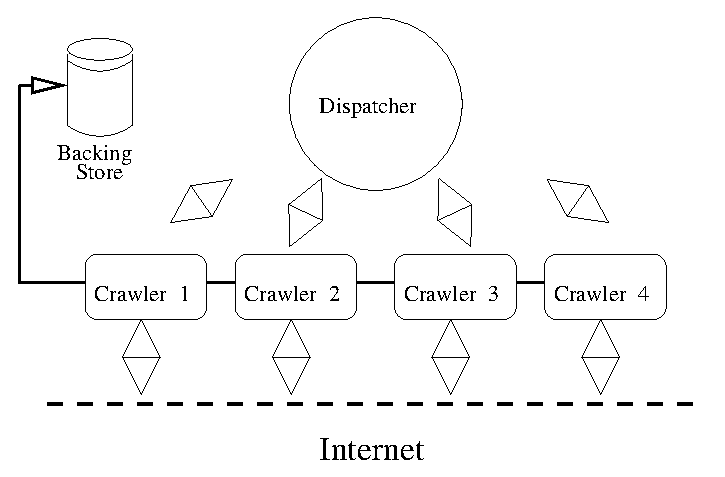
\epsfig{file=./images/crawler_overview.eps, scale=0.75}
  }
  \caption{Architecture Overview}
  \label{fig-architecture}
\end{figure}

\subsection{Implementation}
Labrador is implemented in Perl using object-oriented modules. Perl is not a common development language in this department, however it had several attributes that made it a good choice for writing a crawler:
\begin{itemize}
\item{Firstly, the Comprehensive Perl Archive Network\cite{site1} (CPAN) is the Perl language's open source repository of useful modules. Most modules in CPAN are very mature due to peer usage and review. The archive is very extensive in breadth of modules available. Examples of modules of which I made extensive use: HTML Link Extaction; URL Normalisation; HTTP Fetching; Robots.txt parsing.}
\item{The language's extensive string processing facilities, particularly Perl's regular expression engine.}
\item{Perl's low-level interface to the Unix system calls, which allow very direct manipulation of sockets.}
\item{Not least, my own familiarity with the language. This was massively beneficial, as well as the expressiveness of the language, which allows succinct coding of complex concepts.}
\end{itemize}

\section{Crawler - Dispatcher Communication}
Labrador was designed around minimising network traffic between the dispatcher and the crawlers. One TCP connection is opened between each crawler and the dispatcher. Crawlers ask `questions' to the dispatcher, which processes the question and then `answers' the crawler in an agreed protocol.

\subsection{Network Protocol}
The protocol was design to be easily human readable, while still easy to parse using simple string processing functions or regular expressions. Questions and answers follow the same format: the verbname and the first parameter; followed by optional parameters; the end of the question or answer is marked by a single period followed by a new line. This is shown below:
\renewcommand{\baselinestretch}{1.0}
\begin{verbatim}
VERBNAME argument1
argument2 
argument3
many arguments
last argument number x
.
\end{verbatim}
\renewcommand{\baselinestretch}{1.5}

In `answer' messages, VERBNAME is replaced by a status code from which the client can deduce whether the request was successful or not. Additionally, it is common for argument1 to be a textual description of the status code to allow easier human interpretation of the reply. To anyone familiar with common Internet protocols, it can be seen that Labrador's network communication protocol takes wisdom from several common protocols, mainly the HTTP and the SMTP protocols. The use of a textual protocol ensures that the developer can easily inspect the raw message and ascertain the meaning and content of the message. By using the uncommon character combination of `\textbackslash n.\textbackslash n' as an end marker, it was straightforward to match one message by performing a substitution regular expression, or more simply using a linear string search function to find the sequence. It should be noted that regular expression implementations use the stack heavily and it was found that a 6000 line message exceeds the environment's default stack limit, causing a segmentation fault. Hence, a linear search, such as Perl's index() function, tends to be far faster.\\
\ \\
In Labrador's network protocol, the end of message marker described above (`\textbackslash n.\textbackslash n') came from the end of DATA block in the SMTP protocol\cite{rfc821}. The readable verb names and status codes were inspired by the HTTP protocol\cite{rfc2616}. Verbs can only be called when the calling client has sufficient privilege. Table \ref{tbl-commands} shows the supported commands and their privilege levels, while more in-depth information on the protocol itself can be found in Appendix \ref{appndx-protocol}.


\subsection{Dispatcher Network-level Design}\label{sect-dispnetworkdesign}
I was keen for Labrador's dispatcher to be built as a single-threaded application. There were several reasons behind this: 
\begin{itemize}
\item{Perl's thread support has not yet matured to a level with which I was happy, in particular, not all modules from CPAN are yet thread-safe.}
\item{A single-threaded program can be kept more simple, as there would be no need for complex locking of data structures, ensuring responsiveness and thread-safety.} 
\end{itemize}
Hence, while many crawlers can be connected to the dispatcher simultaneously, the dispatcher can only process one question at a time. However, due to Labrador's typical modus operandi, in which the crawl is partitioned, means that the dispatcher is not a bottleneck of the crawl. Partitioning is further described in \ref{sect-partitioning}.\\
\ \\
It has been standard practice in Unix programs for many years to use `non-blocking sockets' when a process must manipulate multiple network sockets without blocking for reading or writing on any single socket. Non-blocking sockets is a series of system calls which prevent blocking when reading or writing a socket. I based my low-level network code (the Connections module) on the non-blocking sockets example from the Perl Cookbook\cite{book1} (Recipe 17.13). A continuous loop is executed, which polls sockets for new incoming data, processes messages once a whole message has been received and sends as much data on a socket as possible without blocking. I had a problem with the Cookbook's handling of partial sends, so further referred to Unix Networking Programming\cite{book2} to fully understand the system calls involved. It is interesting that the Unix system call interface has changed so little in the last fourteen years, that the first edition was still relevant and that Perl's low-level treatment of sockets is so close to the actual system calls, that example networking source code can easily be migrated from C to Perl.

\subsection{Dispatcher Event Handling}\label{sect-dispevents}
The dispatcher is built on a layered architecture, which can be seen in Figure \ref{fig-disp_events}. The Connections module responsible for the network I/O as described in Section \ref{sect-dispnetworkdesign}, passing events up to the Events module. The Events module handles three primary events: crawler\_connect; crawler\_disconnection; and event\_command. The events module will inform the dispatcher directly of connections and disconnections. However, on a command invocation, the Events module will check to see if the Commands module has registered a command of that name, and if the crawler is privileged enough to execute the command. Different commands require different privilege levels, which is designed to ensure that only clients that are permitted to can peform certain commands. For instance, the dispatcher will not allow a crawl to be stopped unless the client had logged on using the correct administrator privilege password. All protocol commands and their privileges can be seen in Table \ref{tbl-commands}.\\
\begin{table}
\begin{center}
\begin{tabular}{|l|l|}
\hline
\bf{Command Name} & \bf{Privilege Level} \\
\hline
HELO & Any \\
\hline
QUIT & Any \\
\hline
NOOP & Any \\
\hline
CONF & Logged on \\
\hline
MONITOR & Logged on \\
\hline
WORK & Logged on \\
\hline
NEXT & Crawler \\
\hline
FINISHED & Crawler \\
\hline
FAILED & Crawler \\
\hline
ROBOTS & Crawler \\
\hline
ROBOTSFILE & Crawler \\
\hline
STATS & Crawler \\
\hline
FINGERPRINT & Crawler \\
\hline
SHUTDOWN & Crawler \\
\hline
ALLOWED & Crawler \\
\hline
CHECKPOINT & Administrator \\
\hline
PAUSE & Administrator \\
\hline
START & Administrator \\
\hline
STOP & Administrator \\
\hline
\end{tabular}
\caption{Network Protocol - Commands \& Privileges. Further protocol details in Appendix \ref{appndx-protocol}.} \label{tbl-commands}
\end{center}
\end{table}

If the command is permitted, then the correct subroutine is called in the Commands module. Each command subroutine calls the appropriate methods in the Processing module. The command subroutine contains no `business logic' itself - all business logic is contained in the Processing module.

\begin{figure}[h]
  \centerline{
    \epsfig{file=./images/disp_layers.eps, scale=0.75}
  }
  \caption{Dispatcher event processing model}
  \label{fig-disp_events}
\end{figure}

\section{Dispatcher Architecture}
\subsection{Overview}
In Section \ref{sect-dispevents}, I described all the components of the dispatcher below Processing level. The processing module is responsible for all business logic functionality, which includes enqueuing and dequeuing of URLs, filtering URLs and recording their state, as well as recording document fingerprints. The upper-level architecture of the dispatcher can be seen in Figure \ref{fig-disp_layers2}, and will now be described in detail.


\begin{figure}[h]
  \centerline{
    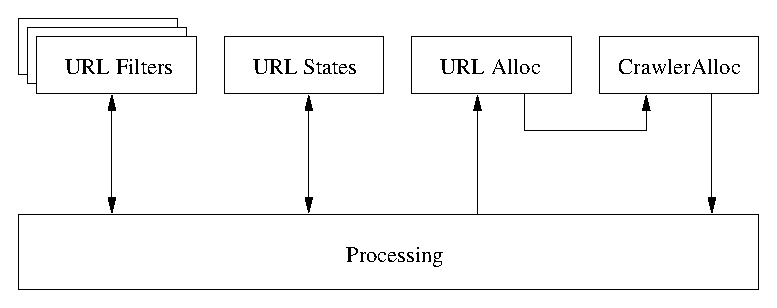
\epsfig{file=./images/disp_layers2.eps, scale=0.75}
  }
  \caption{Dispatcher crawling level components}
  \label{fig-disp_layers2}
\end{figure}

\subsection{URLFilters}
The URLFilter modules are responsible for ensuring that any URLs queued are allowed and within the current crawl domain. URLFilters are discussed further in Section \ref{sect-preventtrapped}. For their use in a production crawl, refer to Appendix \ref{appndx-config}.
\subsection{URLState}
Many papers\cite{ref1,ref2} mention using digests of URLs to minimise the size of the URLState table. Although Labrador's default URLState module does not, it would be straightforward to use a replacement that implements a Bloom filter, such as the Internet Archive crawler uses\cite{ref16}.\\
\ \\
The default URLState implemetation is just a light wrapper around a persistent hash table. Its purpose is to record which URLs are queued or have been fetchedand is used to prevent the crawler fetching any URL more than once.
\subsection{URLAlloc}
The URLAlloc module is responsible for enqueuing and dequeuing URLs onto the dispatchers master queue. Several different implementation exist - Breadth-First queuing, Depth-First queuing and Delay enqueing for Host Delay support. Breadth-first provides the best crawl results\cite{ref8}. Depth-first crawling is seldom used as it tends to become involved in the lower depths of a site before it finishes crawling the upper parts which are generally more important. The implementation of the Delay URLAlloc module (which queues in a breadth-first fashion) is described in Section \ref{sect-hostdelayimpls}. 
\subsection{CrawlerAlloc}
The CrawlerAlloc module is responsible for dequeuing URLs from the master queue then assigning and queuing them to a particular crawler, ready for that crawler's next request. If the crawler is running in partitioned mode, then the Partitioned CrawlerAlloc module must be used.

\section{Partitioning}\label{sect-partitioning}
\subsection{Overview}
To acheive scalable performance, Labrador was written as a distributed crawler, where the workload of fetching and processing URLs are performed by the crawler processes. Labrador has two modes for performing distributed crawling:
\begin{itemize}
\item{Simple\\} 
Simple mode means that each crawler will submit any URLs it found when processing a fetched page to the dispatcher and then ask the dispatcher for the next URL it had to fetch. This mode produces a processing burden on the dispatcher, due to the single threaded architecture used by the dispatcher, because the dispatcher can only process one command at a time. This means, when at high load, the dispatcher becomes the bottleneck for the entire crawling system.
\item{Partitioned\\}
Partitioned mode improves the speed of the system by allowing each crawler an amount of autonomy. Partitions of URLs are allocated to the each crawler and each crawler is permitted to crawl any URLs it finds that are in one of its partitions, without communication with the dispatcher. When a crawler discovers URLs not in its partition, then it submits them to the dispatcher for allocation.
\end{itemize}

\subsection{How Partitioning works}
Cho and Garcia-Molina describe\cite{ref3} three forms of partitioning a crawler: URL-hash based; Site-hash based; and Hierarchical. It should be noted that the URL-hash based forms, while discarded by Cho and Garcia-Molina, are effective in particular setups, such as crawling \{www,ir,www.brc\}.dcs.gla.ac.uk, where Host Delay is not required.\\
\\ \
When operating in partitioned mode, each of Labrador's crawlers, on receiving a URL, will compute the hash for that URL and allocate itself that hash. From then on, only URLs which have the same hash values as previously allocated URLs will be kept on the dispatcher. Others URLs, known as inter-partition links are sent back to the dispatcher for allocation, or to be given to the appropriate crawler if their partition is already allocated.\\
\\ \
Labrador operates as an exchanging crawler\cite{ref3}, which ensures that crawlers do not fetch pages from URLs that are not in its partition, thus nullifying any overlap between crawlers. However to keep optimal coverage, links are exchanged between crawlers via the distpacher. An alternative form, cross-over crawlers, allow crawlers to crawl URLs outwith their own partition, provided they have exhausted their own. In this form, without a high level of communication, there is a risk that different crawlers may fetch the same page. This uses excess resources and requires that the indexer is aware that it should skip URLs that have previously been processed. The final form of partitioned crawlers, firewalled crawlers, do not crawl out-with their own partitions and do not exchange links. This leads to poor coverage of the web, as parts of partitions may only be accessable from other partitions.

\subsection{Paritioning options}
I developed two main forms of partitioning crawls, based on URL-hash based and Site-hash based from above. Each form has several derivatives, as seen in Table \ref{tbl-partitions}.\\
\begin{table}
\begin{center}
\begin{tabular}{|l|l|l|l|}
\hline
\hline
\bf{No.}& \bf{Parition Name} & \bf{Type} & \bf{Supports Host Delay} \\
\hline
\hline
1 & SingleHostDirectory & URL-hash & No \\
\hline
2 & MultipleHostDirectory & URL-hash & No \\
\hline
3 & SingleHostTopDirectory & URL-hash & No \\
\hline
4 & MultipleHostTopDirectory & URL-hash & No \\
\hline
\hline
5 & SeenHost & Site-hash  & Yes \\
\hline
6 & DomainLevel & Site-hash & Yes \\
\hline
\end{tabular}
\caption{Labrador's Partition options}\label{tbl-partitions}
\end{center}
\end{table}

The Directory partition types assign different hash values to different directories, meaning that the crawling of any host could be split across several crawlers. This is why Host Delay is not supported for these Partition types.
\begin{itemize}
\item{SingleHostDirectory:}
This works by calculating the directory path to the file and using that as the hash value. This means that only files in the same directory are in the same partition.
\item{SingleHostTopDirectory:}
This partitioning scheme calculates the top level directory of the URL, so any files crawled in that directory or any subdirectory will be in the same partition.
\item{MultipleHostDirectory \& MultipleHostTopDirectory:}
These partitioning schemes are similar to their Single counterparts, except that the hostname of the URL is prepended to the hash value to ensure that the same directory path on a different host falls in a different partition.
\item{SeenHost:} This partitioning scheme works by ensuring that a crawler will only crawl URLs that have a hostname to which the crawler has been allocated before. URLs found that contain previously unseen hosts are returned to the disptacher.
\item{DomainLevel:} This is an extension of the SeenHost partitioning, where partitions are formed using levels of domain names. For instance, a crawler maybe assigned dcs.gla.ac.uk, while another is assigned arts.gla.ac.uk. This could be extended to form hierarchical crawling partitioning\cite{ref3}, where a master dispatcher may allocate a top-level domain, for instance .uk, to a local dispatcher, which will then further split .uk into smaller partitions to allocate to its crawlers.
\end{itemize}
Table \ref{tbl-partitionsex} gives examples of hash values calculated from sample URLs.
\begin{table}
\begin{center}
\begin{tabular}{|l|l|l|l|l|}
\hline
\bf{URL} & \bf{1} & \bf{3} & \bf{2} & \bf{4} \\
\hline
http://a/b/c/index.html & /b/c/ & /b/ & a/b/c/ & a/b/ \\
\hline
http://z/b/c/index.html & /b/c/ & /b/ & z/b/c/ & z/b/ \\
\hline
http://z/ & / & / & z/ & z/ \\
\hline
http://a/index.html & / & / & a/ & a/ \\
\hline
\end{tabular}
\caption{Hash values of example URLs under different partitioning schemes. URLs not having the same hash value in the set assigned to the crawler are sent to the dispatcher.}\label{tbl-partitionsex}
\end{center}
\end{table}
\ \\
Different alternatives of partitioning schemes may produce different amounts of inter-partition linkage. I evaluate different partitioning schemes in Section \ref{sect-evalpartitioning}.

\section{Crawler Architecture}
\subsection{Overview}
Labrador's crawlers use a layered approach to reduce cohesion between modules - many modules can be replaced by drop-in equivalents provided the same interface is implemented. The Agent module sits at the lowest level and performs all HTTP operations with remote hosts. It is tasked by the CrawlerHandler module, which also has event handlers that the Agent calls back to when the event occurs. The CrawlerHandler module passes the retrieved document to the ContentHandlers which save the content. The CrawlerHandler module also calls the currently loaded Manager module to obtain fresh URLs to be crawled. It is up to the implementor of the Manager module to perform communications with the dispatcher to retrieve the fresh URLs.\\

\begin{figure}[h]
  \centerline{
    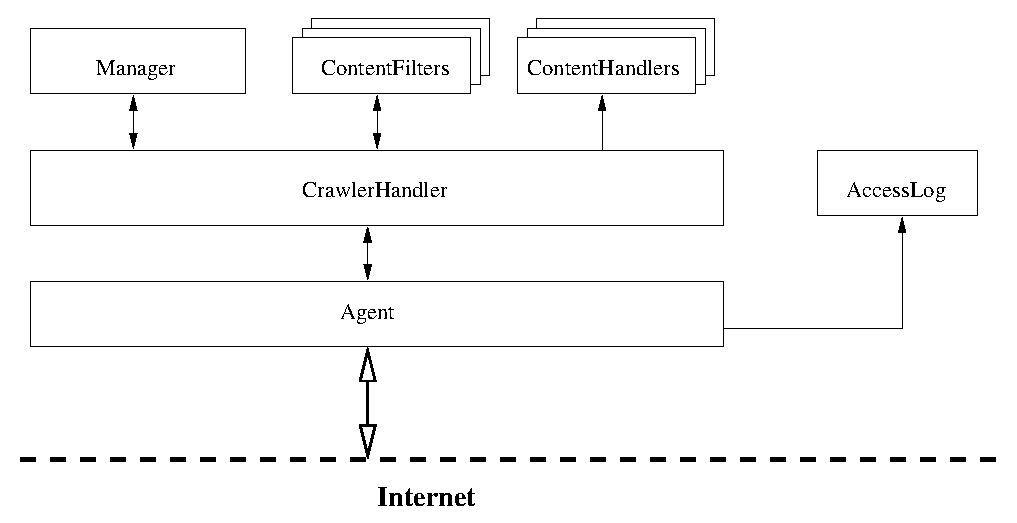
\epsfig{file=./images/crawler_layers.eps, scale=0.75}
   }
\label{fig-crawlerlayers}
\caption{Crawler architecture}
\end{figure}


\subsection{CrawlerHandler}
This is the centre of Labrador's crawler routines. The CrawlerHandler module basically executes a continuous loop, fetching a URL from the currently loaded Manager module and passing it to the Agent to crawl. When given a URL for a host it has not visited before, it will performs robots.txt checks, which may include a robots.txt fetch from the remote host.\\
\ \\
When the Agent finishes fetching a remote page, it calls the appropriate event method provided by the CrawlerHandler: agent\_success; agent\_redirect; agent\_failure. The agent\_success method is the most interesting, as it performs the most critical crawling tasks. Firstly it runs the document through any loaded ContentFilters. These will tell the crawler if it is permitted to follow any links or index the document. If the links can be followed, then any links are passed to the current Manager module. If the document can be indexed, then the document is passed to any loaded ContentHandlers.\\
\ \\
The agent\_redirect method handles redirects by requeuing the target URL of the redirect. The agent\_failure method simply informs the dispatcher that the URL failed. Both methods call event handlers in the ContentHandler modules in case any  wish to handle the redirect or failure cases.

\subsection{Agent}
The Agent module is responsible for lower-level network operations of the crawler (discounting dispatcher communications) and primarily exists to fetch URLs. When a URL is retrieved, the Agent calls the appropriate event handler in the CrawlerHandler, whether the event is a success, redirect or failure. In the case of a success, the Agent will pass back a Document object to represent the downloaded document.\\
\ \\
The libwww-perl modules from CPAN\cite{site1}, that the Labrador Agent uses for all underlying HTTP communications, are very powerful and mature, which keeps the source of the Agent module very clean. Labrador also makes full use of any HTTP extensions available to it. For instance, if the remote server supports HTTP compression, then Labrador will use it and decompress the content before handing to the Document object.\\
\ \\
While each Labrador crawler only supports fetching from one host at once, very little changes would have to be made to the rest of Labrador if the current Agent module was replaced by one which could support non-blocking socket fetches from multiple hosts concurrently. The current Agent implementation only opens one connection at once, and hence the the process is not downloading content while a finished page is being processed. The duration of time that a page is being processed would be ideal for the operating system to be downloading other pages for the same process. In practice, more than one crawler process is normally operating on any crawler machine at one time, and while one process is downloading, another is using the CPU to process a page. However, running multiple processes on one machine is not an optimial design, as each process requires separate memory space, and context switches become a significant overhead. For this reason many crawlers, such as Mercator\cite{ref2} and Googlebot\cite{ref7} use the non-blocking design, opening hundreds of connections per process, but only running one process per machine. Additionally, the disk I/O for saving crawled pages is serialized instead of being interspersed between competing processes, removing another overhead.\cite{book3}.

\subsection{ContentFilters}
The ContentFilters are a suite of modules that permits Labrador to note if a document can be indexed or its links followed. I have implemented five ContentFilter modules, described in Table \ref{tbl-contentfilters}.
\begin{center}
\begin{table}
\begin{tabular}{|l|l|}
\hline
\bf{Name} & \bf{Function} \\
\hline
Binary & Prevents binary content from being indexed. Terrier has no support for binary \\
& content and therefor it just pollutes the index. \\
\hline
ContentTypes & This ensures that Labrador only indexes the content that has a Content-type\\
& header that is desired. \\
\hline
FingerPrint & This is Labrador's duplicate detection module, which uses the MD5\cite{rfc1321}\\
& digest algorithm. This is further discussed in Section \ref{sect-dupdetection}.\\
\hline
MetaRobots & This module parses any meta-robots directives, as discussed in Section \ref{sect-metarobots}.\\
\hline
WhitelistLanguages & This module will let files through only if they contains at least one word \\
& from the specified stopword list. This simple technique is a good indicator\cite{wechsler97multilanguage} \\ & of language, but could be extended to cover all the techniques covered in the paper.\\
\hline
\end{tabular}
\caption{Labrador's ContentFilter modules}\label{tbl-contentfilters}
\end{table}
\end{center}

\subsection{Manager}
The Manager is one of two modules that have been specified to be loaded in the configuration file. These are Simple and Partitioned. \\
\ \\
The Simple module proxies requests from the CrawlerHandler straight to the dispatcher and has very little functionality itself.\\
\ \\
In contrast, the Partitioned Manager module actually replicates some of the functionality from the dispatcher. This is required, because a partitioned crawler has to function without constant communication with the dispatcher. The modules it shares with the dispatcher are: URLFilter, URLState, partitioning schemes and URLAlloc. Without these modules being available on the crawler, the partitioned crawler would not be as fully controlled as it would be under the Simple Manager module.

\subsection{Document handlers}
Document handlers are a suite of modules that handle any specific Content types that have special needs. Currently the types are HTML, Postscript, RTF and PDF files, although other classes could easily be written for say Microsoft Word or Powerpoint documents. The document handler for a type is responsible for converting the document, should it not be indexed in its current form (for instance PDF and Postscript documents), and performing link extraction on the type if possible.

\subsection{ContentHandlers}
Finally, the ContentHandler are the last link in the chain, where content is saved. Labrador has only been used to save documents for one indexer - the Terrier framework, so only one module has been developed here. The PreTerrier module saves the content in the way that exactly matches the needs of the Terrier indexer.

\section{Configuration File}
Although not particularly notable themseles, the Config module and the Labrador configuration file allow Labrador to be extremely flexible. Over the development of Labrador, I have matured a set of configuration files for specific crawls. To change a Labrador instance over to a different crawl, simply means specifying a different configuration file on the command line. As each crawler is started, it obtains its configuration file directly from the dispatcher - it has no need for a local copy of it. A sample configuration file is available in Appendix \ref{appndx-config}.\\
\ \\
When developing Labrador, the Config module was an early milestone, which meant that from then on any parameter that could be obtained from the configuration file was obtained, even if a default was set.


\chapter{Politeness}\label{chp-polite}
\section{Overview}
Politeness is suite of policies and de-facto standards. Essentially, they exist to prevent a crawler annoying the webmaster of a site its crawling. This might happen for a number of reasons:
\begin{itemize}
\item{The crawler is accessing parts of a website the webmaster would prefer it didn't.}
\item{The crawler is accessing to website at too high a speed.}
\end{itemize}
Annoying a webmaster is counter-productive, because they may prevent the crawler from accessing their website in the future. This means that the content cannot be crawled and hence the index cannot deliver results from those pages.

\section{Robots Exclusion}
\subsection{Background}
There are two forms of Robots Exclusion protocol that crawlers must obey. Firstly, the robots.txt\cite{site4} file allows the webmaster of a site to place control over what pages a web crawler will fetch. Secondly, the meta-robots directive\cite{site5} in the HTML source of a page will provide essentially the same control.
\subsection{robots.txt}
The robots.txt\cite{site4} protocol is a file which a crawler must first fetch from each host before it crawls the host. Although its presence is optional, the crawler must fetch http://hostname/robots.txt and parse the file to recognise the rules it contains. Below can be found an example of a robots.txt file.
\renewcommand{\baselinestretch}{1.0}
\begin{verbatim}
#robots.txt file from http://www.dcs.gla.ac.uk/
User-agent: *
Disallow: /cgi-bin/
Disallow: /people/
\end{verbatim}\\
\renewcommand{\baselinestretch}{1.5}
Each robots.txt file has list of rules which specifies which directories may not be crawled by any crawler. It can also specify, using the User-agent directive, any directories exclusions specific to a particular crawler. In the example, no crawlers are permitted to fetch any URLs starting http://www.dcs.gla.ac.uk/cgi-bin/ or http://www.dcs.gla.ac.uk/people/.\\
\ \\
When any crawler of Labrador finds a host it has not visited before, it checks its local robots.txt cache to see if a copy of the robots.txt file has been downloaded. If this is not the case, then the dispatcher's robots.txt cache is checked as well, before downloading the file itself. When any crawler downloads a robots.txt file, it will send a copy of the file to the dispatcher to be added to the global cache. By default, Labrador caches robots.txt files for 25 days, although this can be altered by the RobotsTxtExpiry in the configuration file.
\subsection{Meta-Robots}\label{sect-metarobots}
The Meta-Robots\cite{site5} specifies an alternative to the robots.txt standard, which is specified in a meta tag in the HTML of the page. Traditionally meta tags have been used to specify other meta data for a search engine to use during the indexing phase, such as document keywords or a description, but soon after the robots.txt standard was introduced, the web authors wanted more fine-grained control than the robots.txt file provided. The meta-robots standard allowed web authors to specify whether a crawler should index a page without having to change the robots.txt file. This was particularly useful when the author of the document did not have control over the robots.txt file of the server they were using - for example a shared hosting environment.
\indent \begin{verbatim}<meta name="robots" content="noindex">\end{verbatim}\\
Above is an example meta-robots directive that specifies that a crawler may not index that page. The values supported by the meta-robots directive is shown in Table \ref{tbl-metarobots}.
\renewcommand{\baselinestretch}{1.0}
\begin{table}
\begin{center}
\begin{tabular}{|l|l|}
\hline
\bf{Directive} & \bf{Description} \\
\hline
none & A crawler may not follow links from this page, nor index the contents.\\
\hline
noindex & A crawler may not index the contents of this page \\
\hline
nofollow & A crawler may not follow links on this page \\
\hline
all & A crawler may index this page and follow its links \\
\hline
\end{tabular}
\caption{Meta-Robots directives}\label{tbl-metarobots}
\end{center}
\end{table}
\renewcommand{\baselinestretch}{1.5}

\section{Host Delay}
\subsection{What is Host Delay?}
Host Delay (or per-host delay) relates to the directive in Labrador's configuration file that specifies the delay in seconds between each request to a given host. It is part of the politeness protocols, because by crawling a host too fast, the crawler is likely to annoy the server's webmaster:
\begin{itemize}
\item{Uses bandwidth which costs the webmaster's organistion.}
\item{The crawl may be mistaken for a Denial of Service attempt.}
\item{Otherwise interfere with the day-to-day running of the website. For instance, the site may become slow because of the crawler, thus detracting potential customers.}
\end{itemize}

\subsection{Why is Host Delay a problem for a crawler?}
There are two essential problems with Host Delay:
\begin{itemize}
\item{An efficient implementation that correctly queues URLs, such that the delay is respected, is complex to develop.}
\item{The amount of time that it adds to a crawl, compared to crawling the same site with no delay.}
\end{itemize}


\subsection{Host Delay queuing implementations}\label{sect-hostdelayimpls}
I attempted several queuing implementations before I found a solution which was both correct and efficient.
\subsubsection{Re-queuing of URLs}
My first attempt at implementing a per-host delay system involved pushing URLs that were deemed too early back into the queue, at a place thought to be approximately correct. I tried this using two different heuristics:
\begin{itemize}
\item{Using the current URLs/sec rate to approximate a position in the queue.}
\item{Using the current URLs/sec rate and the position in the queue of the most recent URL seen for that host.}
\end{itemize}
Both these heuristics were found to be inefficient. This was primarily due to locality in links found on HTML pages (most sites link to pages in their own site\cite{ref17}), which meant that queues tended to consist of groups of URLs for the same host. The algorithm would push each URL back as far as it thought it needed to be in the queue to cause host delay. However, the crawler would end up working through all URLs at the head of the queue, without finding a URL that was ready to be fetched.

\subsubsection{Queues for each second of delay and queue promotion}
Another implementation I attempted was to use a set of arrays, each array representing x-many seconds of delay. URLs were sorted onto an appropriate delay array, based on how much the previous URL for that host was delayed and when that event ocurred. Once every second, each queue was promoted - i.e. queue 4 became queue 3, queue 5 became queue 4 and so on. This prevents URLs from being fetched before they are ready.\\
\ \\
\begin{figure}[h]
  \centerline{
    \epsfig{file=./images/slicedqueue.eps, scale=0.7}
  }
  \caption{Sliced Queue}
  \label{fig-slicedqueue}
\end{figure}
\ \\
This implementation was found to be inefficient, as when crawling on an institution scale, the crawler was often delaying URLs by tens of thousands of seconds of delay and hence requiring tens of thousands of separate queues. At this size, the overhead of promoting all the queues once each second became critical. This problem could have been eliminated using a renumbering of the queues during promotion instead of moving data between queues. However, this was deemed less favourable than an attempt at using DelayLines, as described below.

\subsubsection{DelayLine of URLs}
A DelayLine\cite{site1} is a sorted array where each element has a `not before time' tagged onto it. De-queuing is a constant-time operation, while inserts are O(nlog n). At first I tried using a DelayLine for all URLs in the system, delaying each URL based on the amount of delay the previous URLs has had (or time since last fetch if no other requests for that host are currently queued). However, again as the delayline for single crawler became nearer 40,000 URLs for a medium size crawl, the insert operation became prohibitively expensive. I could have improved the insert operation to O(log n) time, but then deemed that this would not provide the level of performance required.

\subsubsection{DelayLine of Hostnames and queues for each hostname}
My final implementation of a per-host delay data structure was using a separate queue for each host of the crawler and a DelayLine, as described above, to provide the delaying of each host. This can be seen in Figure \ref{fig-delaylinehosts}. The URLAlloc Delay module dequeues a hostname that is ready for every request by the crawler Manager. Being ready means that the time since the last fetch from that host exceeds the Host Delay setting. This dequeued hostname tells the Delay module from which queue it should next dequeue a URL. If the DelayLine has no hosts that are ready to fetch, then the crawler will determine how long it has to wait and if no URLs are available from the dispatcher, then the crawler will sleep until there are some ready. Due to the fact that there are few hosts active for a crawler at any one time, this implementation is as efficient as desired and correct, in as much as it prevents URL fetches before they are ready.

\begin{figure}[h]
  \centerline{
    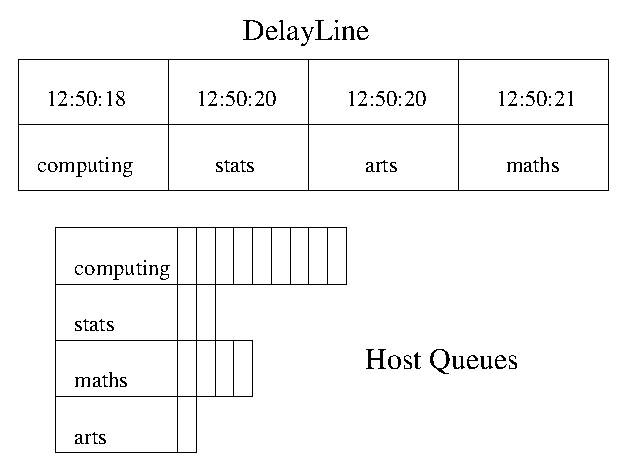
\epsfig{file=./images/delayline_hosts.eps, scale=1.0}
  }
  \caption{Delay internals: Host queues and a DelayLine of hostnames.}
  \label{fig-delaylinehosts}
\end{figure}

\subsubsection{Approximate permutations of URLs into chunks}
Many crawlers use hashing functions, e.g. $k$-way unshuffle permutations\cite{ref1}, to group URLs into chunks, which have enough URLs of different hosts in each chunk to ensure that the crawler will be kept busy without fetching from any one host too often. This method has the advantage that no sorting needs to be done at insert time, and overheads are minimised as URLs are chunked. I believe that each chunk of URLs would still have to be marked with a time that it cannot be fetched before, because towards the end of a crawl when the crawler were running out of hosts, they might run through the chunks too quickly, resulting in insufficitently delayed requests.
\subsection{Host Delay time issue}
Once a few crawls have been performed by a crawler that correctly implements a Host Delay functionality, it becomes apparent that the rate at which URLs can be fetched could be severly hampered. Adding more crawlers does not improve the URL rate. Quite simply, the crawlers do not have enough work to keep them `entertained'. This means that at a given time during a crawl, some crawlers may be asleep, as they have recently fetched from all their allocated hosts. They are not permitted to fetch from any host until the Host Delay has expired for that host. They may try asking the dispatcher if it has any more URLs it can give it, but often this is not sufficient to keep them busy.\\
\ \\
In fact, the time taken to completely crawl a domain ($T$), can be expressed as:
\ \\
\indent $T \geq HostDelay \times (size\ of\ largest\ site\ in\ domain)$
\ \\
Note that this is irrespective of the number of crawlers, or of the size of the domain.
Due to this, during a typical crawl the URL rate diminishes towards the end of the crawl, as more and more sites have had all their discovered pages retrieved.\\
\ \\
Empirically, let's examine the domain gla.ac.uk:

There are 200 sites with less than 100 pages and only 4 with greater than 30,000 pages, ignoring manually blacklisted spider traps. With a Host Delay of 3 seconds, any crawl of of gla.ac.uk can be no shorter than 30,000 * 3 seconds, i.e. 25 hours. Note that increasing the number of crawlers may increase the fetch rate when the crawlers are backlogged, but will have no effect on the minimum crawl time. However, normal crawls take longer than the minumum, as explained in Section \ref{sect-discovery}.
\ \\
Interestingly, the distribution of host sizes versus frequency follows a power-law distribution, as can be seen in \ref{fig-hostsizedistribution}. This graph was drawn using host sizes found during crawls of the universities of Glasgow, Strathclyde, Paisley and Glasgow Caledonian. A larger crawl may produce a clearer distribution, as documented by Huberman and Adamic (1999)\cite{ref15} who used information from crawls by Alexa and Infoseek.

\begin{figure}[h]
  \centerline{
    \epsfig{file=./images/log_e.ps, height=5in, angle=-90}
  }
  \caption{Distribution of host size versus frequency}
  \label{fig-hostsizedistribution}
\end{figure}

\subsection{Discovery period}\label{sect-discovery}
In the formula above, the reader should note that I have stated $\geq $ and not a direct equality. This is due to what I have determined to be the discovery period. This essentially comes in two varieties, host discovery and URL discovery.\\
\ \\
For example, for a crawl of the gla.ac.uk domain seeded with just the University homepage, http://www.gla.ac.uk/, where every page in the domain is eventually reachable from the homepage, the URL rate at first will be poor, but will increase as more hosts are discovered. This means that the crawlers spend less time idle waiting to be allowed to access their allocated hosts again.\\
\ \\
Similarly, a site may only be half crawled by a crawler, as the site may happen to have its links partitioned into n-partite sections. The next section will only be discovered when crawling another separate site. If this is a big site then valuable time will have been lost in the gap between one partition of the site being finished and another one being discovered. This is the problem of URL discovery.\\
\ \\
Discovery period can be minimised when doing subsequent crawls of a domain by seeding the crawler with all URLs fetched during the previous crawl. This means that the host and URL discovery period will be mostly eliminated, although new hosts and URLs since the previous crawl still have to be discovered. This immensly speeds up the initial URL fetch rate and is the most effective way of speeding up a crawl, apart from shortening the host delay. Most commercial search engines seed their crawlers with URLs of the previous crawl to minimise the discovery period effect (Google prioritises the URLs by PageRank as well\cite{ref5}).


\chapter{Crawling Challenges}\label{chp-challenges}
\section{Crawler Traps}
\subsection{What is a Crawler trap?}
A crawler trap is a site which the crawler may enter and be unable to `escape', meaning that the site keeps generating new links for the crawler to explore. These are most often dynamic sites, where pages are generated in response to each request. Below I have described several common examples of crawler traps:
\begin{itemize}
\item{Recursive symbolic links\\}
A simple crawler trap can be generated by symbolically-linking an entry in a Unix web-accessable directory to the directory itself. The crawler will enter the directory and follow all the links in the directory, recursing infintely deep into the directory structure.
\item{Calendar applications\\}
During test crawls of the gla.ac.uk domain, the crawler discovered several calendar controls on diary or blog type websites. These formed crawler traps as each calendar would have a link to the previous and following months. In one case, the calendar was good until the year 21,000! Obviously having to crawl 20,000 extra URLs with negligible difference in content adds to the crawling time.
\item{Large web-accessable databases\\}
Crawlers can also become trapped in the websites of large databases. During crawls of university domains, I manually blacklisted the sites of the universitys' library. This was usually necessary as the libraries' web site provide access to their databases of books. In the case of the Glasgow University Library, this meant a site with a page for each of the 2 million books in its collection. Two million requests to the same host, with 3 seconds between each (Host Delay), meant that the site would have taken over 70 days to crawl. When deciding to blacklist a site, the crawler operator should take into account how much information would be excluded from the index, preventing users from finding content that site.
\end{itemize}

\subsection{Preventing becoming trapped}\label{sect-preventtrapped}
Labrador has a very flexable suite of URLFilter modules, which allow very fine grained control of those URLs which are allowed and those which are not. These include white and black lists; regular expression matching on any part of the URL; URL Depth; and URL Length. The Depth and Length modules are effective at filtering out crawler traps. For instance, a URL longer than 1000 characters, or more than 20 directories deep, are not likely to be important. I filtered out most calendar traps by matching for URLs containing the word `calendar' in the querystring. For URLFtiler use in a production crawl, refer to Appendix \ref{appndx-config}. \\
\ \\
Finally, I have implemented an additional filtering of URLs at the crawler, which can be configured to allow only the fetching of a given number of URLs that have exactly the same filename but differ in their querystring component - for example http://a/b?p=1 and http://a/b?p=2. This has turned out to be an effective method of preventing the crawler becoming too deeply involved in a large web-accessable database as described above. By inspection we can see that Google performs a similar process, as the query `site:eleanor.lib.gla.ac.uk' states `about 19,100' results, but this is not a limit of pages on any host, as they query `site:www.bbc.co.uk' finds over 600,000 results. The first site is a web-accessable database with about 1 million records accessed using querystring based URLs, while the BBC website contains primarily static pages.\\ \
\\
Even so, a crawl should be monitored to see where the majority of requests are going. Traps can often be identified by inspecting the logs in realtime. My first crawls were monitored all the time, to ensure they were not crawling sites where they were not permitted, or becoming involved in traps.

\section{Duplicate Detection}
\subsection{Why should we detect duplicates?}
Many documents on the Internet are available under different URLs, meaning that the crawler can not detect before visiting a URL whether it has seen the content before or not. This may be because a server has been mirrored in a different location for fault tolerance reasons, or the same server is known under a different name, or the content may have been copied to a different URL and the original not removed.\\ \
\\
All of these conditions can cause the crawler to download the same page at a different location, unless the content can be identified as identical to previously downloaded pages. If the crawler downloads more than one copy of the same page, this will probably lead to each of the identical pages being weighted the same in a query, leading to result pages containing consecutive runs of essentially identical pages, which lowers the precision of the search engine, e.g. the TREC search engine competition penalises duplicates in results. If duplicate pages are identified, only one copy should be saved for indexing. Additionally, links should not be extracted from duplicate pages, as they will lead to URLs that have already been seen (by absolute URLs), or to URLs not seen, but content that has been seen (by relative URLs).\\
\ \\
Commonly, message digests (hashes) are used to identify the content of a document, as it would be too expensive to identify duplicates using the actual content of the documents. There are two forms of digests, described below.
\subsection{Exact-duplicate detection}\label{sect-dupdetection}
Labrador uses the MD5 digest algorithm\cite{rfc1321} to detect exact-duplicate documents. For each document downloaded, the digest is calculated and passed to the dispatcher. The dispatcher takes a note of the digest and sees if it already has the digest, using a hashtable lookup. The dispatcher records the digest if it has not been seen and informs the crawler of the status of the digest. If the dispatcher has seen the digest before, then the document is discarded, any links found are not extracted and the content is not saved.\\
\ \\
The dispatcher uses GDBM's persistent hashtable for storing the digests. This means that the entire hashtable does not need to be kept in memory, while still providing O(log n) lookups.
\subsection{Near-duplicate detection}
Mercator\cite{ref2}, suggest using Broder's\cite{ref11,ref12} method (Shingling) of producing fingerprints for web pages. Broder's fingerprints collision rate (the probability of two different strings having the same fingerprint) is provable, unlike digest algorithms such as MD5 or SHA. More importantly, Broder's fingerprints can be used to detect near-duplicate documents, such as two web pages with the same content, but different links which is clearly an advantage.\\
\ \\
Labrador does not have support for near-duplicate document detection, but provides a ContentFilter interface which would allow a near-duplicate detection module to be easily implemented.


\chapter{Integration}\label{chp-int}
\section{Outline}
The current departmental search engine which I was to replace is based on the htDig engine, an open source simple matching engine. My brief stated that Terrier, as described in Section \ref{terrier_desc}, was to form the basis of the new website search engine. Although the search functionality provided by Terrier was fast and maturing quickly, no work had yet been done on making Terrier accessable from a webpage. Additionally, it was crucial that a format was developed such that Terrier was able to parse the files of content saved by Labrador during a crawl.

\section{htDig}
The Department of Computing Science website has been using the now outdated HTTP search engine known as htDig\cite{web1} for providing its search results to users. htDig provides basic search functionality, with a combination of algorithms: exact, soundex, metaphone, stemming and synonyms.\\
\ \\
However, htDig lacks certain key abilites that are important in the current generation of search technology:
\begin{itemize}
\item{The ability to crawl and index documents which are not HTML or plain text. This was a fundamental part of my project due to the high frequency of Adobe Acrobat (PDFs) and Postscript files on websites.}
\item{It lacks any modern link-analysis, such as the PageRank\cite{Lawrence981} algorithm used by Google\cite{ref7}. Link analysis is cruical for indentifying authoritive sites for a given topic.}
\item{Finally, htDig lacks performance and ease of configurability.}
\end{itemize}	

\section{Terrier}
\subsection{Crawls}
To ensure that Terrier was correctly able to index the web pages Labrador saved, I had to interact with the Terrier developer, to meet his needs. It was decided to primarily follow the indexing format used by the DOTGOV\cite{site2}, WT2G and WT10G\cite{site3} collections, from the TREC competition, with some extensions. The format is given below.
\renewcommand{\baselinestretch}{1.0}
\begin{verbatim}
<DOC>
<DOCNO>G00-00-0000000</DOCNO>
<DOCHDR>
http://www.aspe.hhs.gov
HTTP/1.0 200 OK
Date: Wed, 30 Jan 2002 17:00:23 GMT
Server: WebSitePro/3.0.37
Accept-ranges: bytes
Content-type: text/html
Last-modified: Fri, 18 Jan 2002 19:04:17 GMT
Content-length: 8228
</DOCHDR>
...Document content...
</DOC>
\end{verbatim}
\renewcommand{\baselinestretch}{1.5}
Labrador also provides links and redirect data files, which make link analysis, such as PageRank\cite{Lawrence981}, easier for Terrier to perform. Links files contain the outgoing links and anchor texts of each link on every page of the crawl, while the redirect files contains a list of redirects found during the crawl. The links files assists Terrier by performing the link extraction it would have had to perform itself, while Labrador has already performed it. Redirect files assist link analysis by identifying slightly incorrect links, e.g. a link to http://a/b can be seen as http://a/b/ which is what it was intended to be, because the former URL redirected to the latter.

\subsection{Matching Models}\label{sect-terriermatching}
Terrier provides nearly 50 matching models, including many Divergance from Randomness (DFR) models\cite{ref14}. However, Terrier has been optimised for the Poisson-based PL2\cite{ref13,ref14} model, as shown below, and it is this model that Terrier uses for the collections I have crawled.\\
PL2: \indent \begin{equation}\label{pl2} w(t,d) = \frac{1}{tfn +1}(tfn \cdot \log_2 \frac{tfn}{\lambda} + (\lambda + \frac{1}{12.tfn} - tfn) \cdot \log_2 e + 0.5 \cdot \log_2(2\pi \cdot tfn))\end{equation}\\
where $tfn$ is the normalised term frequency. It is given by the
%\emph{normalisation 2} \cite{amati03thesis}:
\begin{equation}\label{eNormalisation2}
    tfn=tf\cdot\log_2(1+c\cdot\frac{avg\_l}{l})
\end{equation}
\ \\
He and Ounis\cite{ref13} describe a method where the parameters of the DFR matching model can be optimised pre-retrieval for queries of different clusters. In Section \ref{sect-evalpl2}, I shall show how the parameters for the PL2 matching model required altering as the size of the collection grew.

\section{Using Terrier as a HTTP search engine backend}
A requirement of my project was that Terrier should provide the search results for the departmental websites. To this end, although fast, Terrier only had interfaces for searching its indexes in a batch mode. Hence the first challenge was to provide a suitable API to Terrier via client code.

\subsection{HTTP querying Terrier}

When initialised with a large index, Terrier can be a large, resource heavy system. Hence I deemed it unsuitable to run on the department's main webserver, where it would use more than its fair share of memory and disk space. Therefor I separated the rendering of the results from the querying of the index. This meant that Terrier should be run as backend on a suitable departmental server, while only a small light frontend script would run on the main webserver. The frontend would be responsible for rendering the results to HTML and caching results of queries. This meant that the loading of the main departmental webserver was minimised.\\
\ \\
The best inter-machine protocol, is of course HTTP and I decided that Terrier should be queried for a set of results as shown:\\
\indent http://wokam.dcs.gla.ac.uk:8000/servlet/terrier?q=information+retrieval
\ \\
Of course, a custom network protocol could have been devised, or an alternative technology such as RMI could have been used to effect the inter-process communication across the network. However, RMI would have required that the frontend was written in Java. Alternatively, to design and implement a custom network protocol would have added extra development time that was unnecessary.\\
\ \\
\subsection{XML Results}
When called as shown above, Terrier renders all its results for the query to an XML page. XML was chosen as there are parsers available for all languages on most platforms (from Perl and Python, to Java and C), meaning it enforced no restriction on the implementation of the frontend.\\
\ \\
Furthermore, XML allows a hierarchical data structure, as opposed to a flat data format, as would likely have been produced with a textual data format. Hierarchical data format would be useful in this context if results were required to be grouped hierarchically in some way. Some search engines do similarly for `Similar Pages' results.\\
\ \\
In Terrier's XML schema, some fields are optional, for example the description tag which is only produced if the Meta Indexer module managed to produce an description for the document. Due to the nature of XML, the schema can be extended in the future and existing client applications will ignore tags of which they have no knowledge. Other XML technologies, such as XSLT, allow further flexibilty with the Terrier results in the future.\\
\ \\
When a query is entered, the frontend calls the Terrier backend over HTTP to retrieve the results the first time only. After that, the XML is cached on the webserver by the frontend script. As many queries provide many more results that could be fitted on one HTML page, this saves the frontend calling Terrier to retrieve results number 11-20 etc.\\
\ \\
The XML format that Terrier returns was agreed between the Terrier developer and myself. It provides a rich interface into the results provided by Terrier. Results scores, matching type used, URL, document titles and descriptions are provided in the XML. The Terrier DTD can be found in Appendix \ref{terrier_dtd}.\\

\renewcommand{\baselinestretch}{1.0}
\begin{verbatim}
<terrier>
  <query method="PL2b7.0">iadh ounis</query>
  <results count="333">
  <result number="0" docid="D13-25-50">
    <score>21.710036430488714</score>
    <url>www.dcs.gla.ac.uk/~ounis/bib.html</url>
    <title>Iadh Ounis Selected Publications </title>
    <description>Iadh Ounis Selected Publications Legal notice The documents 
    distributed by this server have been provided by the contributing authors
    as a means to ensure timely dissemination of scholarly and technical work
    on a noncommercial basis.Copyright and all rights therein are maintained
    by the authors or by other copyright holders,</description>
  </result>

  <result number="1" docid="D13-25-48">
    <score>20.265398126400385</score>
    <url>www.dcs.gla.ac.uk/~ounis/bibbooks.html</url>
    <title>More Articles </title>
    <description>More Articles Legal notice The documents distributed by this
    server have been provided by the contributing authors as a means to ensure
    timely dissemination of scholarly and technical work on a noncommercial 
    basis. Copyright and all rights therein are maintained by the authors or 
    by other copyright holders,notwithstanding that </description>
  </result>

  <result number="2" docid="D13-25-49">
    <score>19.200592430026365</score>
    <url>www.dcs.gla.ac.uk/~ounis/bibreports.html</url>
    <title>Iadh Ounis Selected Publications </title>
    <description>Technical Reports and Draft Publications Legal notice The 
    documents distributed by this server have been provided by the contributing
    authors as a means to ensure timely dissemination of scholarly and technical
    work on a noncommercial basis.Copyright and all rights therein are maintained
     by the authors or by other copyright </description>
  </result>

  <result number="3" docid="D12-36-41">
    <score>18.089029243406326</score>
    <url>www.dcs.gla.ac.uk/ir/terrier/publications.html</url>
    <title>Terrier Publications </title>
    <description> The following publications are the result of the development of
    Terrier Vassilis Plachouras,Iadh Ounis and Gianni Amati.A Utility-oriented Hyperlink
    Analysis Model for the Web.In Proceedings of the First  Latin Web Conference Santiago,
    Chile,2003.Ben He and Iadh Ounis.A study of parameter tuning for term </description>
  </result>
  
  <result 
....
  </result>

</results>
</terrier>
\end{verbatim}
\renewcommand{\baselinestretch}{1.5}
The XML format also has optional fields, allowing additional features such as spelling correction to be provided by the frontend only when Terrier suggests it (and it is enabled).

\section{Frontend}
The frontend is responsible for querying Terrier by HTTP, parsing the XML results that Terrier returned and filtering the results down to only those needed for the current page. It then generated a data structure that was combined with a template to produce the resultant HTML page.\\
\ \\
The frontend also cached XML results for a query to its local disk (using the GDBM persistent hash library), so that the frontend had no need to re-query Terrier to retrieve results for subsequent pages of a query. The frontend provides a simple CGI API, allowing the web developer some flexability in how results are rendered, described in Table \ref{tbl-frontendparam}. A screenshot of the front end can be seen in Figure \ref{fig-frontend}.
\begin{table}
\begin{center}
\begin{tabular}{|l|l|}
\hline
\bf{Variable name} & \bf{Description} \\
\hline
query & Search engine string to search for \\
\hline
startpage & Page number to display \\
\hline
perpage & Number of results to put on one page \\
\hline
template & Which of the allowed templates to use to render the results \\
\hline
\end{tabular}
\caption{Querystring CGI Parameters provided by the Frontend}\label{tbl-frontendparam}
\end{center}
\end{table}
\subsection{Templates}
I built the frontend CGI scripts to use HTML templates. This means that no actual HTML code is embedded in the actual source code of the scripts. These have several advantages, listed below:
\begin{itemize}
\item{Development on source code and templates can be done separately, given a stable template API.}
\item{The client-side developer need not know how to program in the language of the CGI script.}
\item{Alternate templates can be used without modifying the source code-base. This is as simple as changing the template CGI parameter, as described above.}
\item{The source code is simpler and clearer because there is no extraneous code related to rendering.}
\end{itemize}
The fundamentals behind using an HTML templating language is that the template file includes the majority of the HTML source. The variables names within the template file are substituted with the data of the same name that is passed to the templating engine. Further flexibility is available by the introduction of features such as file includes, loops and conditional branches. Template variables and loops are passed to the templating engine as hash tables and arrays.

\subsection{Other Features}
The frontend has support for additional features, which are also provided for in the XML schema, but not currently implemented in Terrier. An example of this is the support for query suggestions. Sau Kwan Chan has recently been working on methods for correcting misspelt words in queries. My frontend CGI scripts will render query suggestions to the HTML, if there are any. At time of writing, Sau's suggestion work is not yet sufficiently mature to be integrated with Terrier on a production installation.
\begin{figure}[h]
  \centerline{
    \psfig{figure=images/frontend.eps,height=9in}
   }
\label{fig-frontend}
\caption{Frontend using DCS Skin}
\end{figure}


\chapter{Evaluation}\label{chp-eval}
\section{Overview}
To ensure that Labrador peforms correctly, I ran a series of statistical analyises on my evaluation crawls. These were designed to measure the effects of different partitioning schemes on the crawl and to compare these crawls to a run of Labrador in simple mode.

\section{Problems when evaluating crawlers}\label{sect-evalprobs}
It is particularly difficult to scientifically evaluate a web crawler. This eesentially stems from the fact that it is difficult to create a test environment. Although I ran many test crawls over different sizes of crawl domains, I restricted evaluations crawls to the websites of my department. This was because the amount of change of the website in any given time period is fairly small, meaning there is some hope that if two identical crawls were ran consecutively, they would produce the same results. I found that even in the departmental websites, a fluctuation of URLs fetched could vary between subsequent crawls in one day. This could be caused by additional pages being fetched, or by occasional transient errors created by the webserver under high load - typically this crawl runs at up to 55 URL/sec (averaged over a minute).\\
\ \\
Another external issue that affects the outcome of the crawl is the background network load and server load being experienced during the duration of the crawls. While a crawl may last a couple of hours, network usage may vary from hour to hour (e.g. higher usage during lunch time), and from day to day. This may adversly affect the crawl, but any effect is difficult to measure.

\section{Partitioning}\label{sect-evalpartitioning}
\subsection{Background}
As dicussed in Section \ref{sect-partitioning}, I implemented two modes for Labrador to operate in: Simple; and Partitioned mode. This set of evaluation was performed to compare the crawler over. Three crawls were operated, as described in Table \ref{tbl-partcrawls}.\\
\begin{table}
\begin{center}
\begin{tabular}{|l|l|l|}
\hline
\bf{Name} & \bf{Mode} & \bf{Partitioning} \\
\hline
Crawl 1 & Simple & N/A \\
\hline
Crawl 2 & Partitioned & MultiHostDirectory \\
\hline
Crawl 3 & Partitioned & MultiHostTopDirectory \\
\hline
\end{tabular}
\end{center}
\caption{Evaluation Crawls}\label{tbl-partcrawls}
\end{table}

Each crawl was seeded with only six URLs, the six departmental home pages. They are listed in Table \ref{tbl-smallseeds}.\\
\begin{table}
\begin{center}
\begin{tabular}{|l|}
\hline
\bf{URL} \\
\hline
http://www.dcs.gla.ac.uk/\# \\
\hline
http://www.brc.dcs.gla.ac.uk/\# \\
\hline
http://tlc.dcs.gla.ac.uk/\# \\
\hline
http://ir.dcs.gla.ac.uk/\# \\
\hline
http://grumps.dcs.gla.ac.uk/\# \\
\hline
http://faraday.dcs.gla.ac.uk/\# \\
\hline
\end{tabular}
\end{center}
\caption{Evaluation Crawl - Seed URLs}\label{tbl-smallseeds}
\end{table}


\subsection{Crawl time}
Figure \ref{fig-crawlgraphs} shows URLs fetched by the crawls described in Section \ref{tbl-partcrawls}. It clearly shows that Crawl 3, using the MultiHostTopDirectory scheme was the fastest. The Simple mode crawler was the slowest.\\
\ \\
I expected the Simple mode crawler to be the slowest, as each crawler (8 in this case) must communicate with the dispatcher between every URL. This creates a bottleneck at the dispatcher. MultiHostTopDirectory performed best as its partitions are larger, meaning less inter-partition linkage. When a crawler discovered a link outwith its own partition it has to send it back to the dispatcher. For instance, each lecturer has their home page at http://www.dcs.gla.ac.uk/$\sim$username/. I theorise that most of the links in each lecturers home page create to their own material, which when using MultiHostTopDirectory is in the same partition. However under MultiHostDirectory, sub-directories are a different partition, which means that those links must be sent back to the dispatcher.\\
\ \\
The astute reader may notice that the three crawls did not fetch the same number of URLs, for the reasons described in Section \ref{sect-evalprobs}. Furthermore, all three crawls suffered a drop in rate at approximately 50,000 URLs (although less prononuced in Crawl 3). I theorise that crawls of the departmental website become involved in the Bibliography database around that point. As each bibliography page requires a database fetch, the time taken to fetch the rate is higher, which ultimately affects the fetch rate. Further investigation would be required to validate this theory.
\begin{figure}[h]
  \centerline{
    \epsfig{file=./images/finished.ps, scale=0.60, angle=-90}
   }
\caption{Comparision of Crawls 1, 2 \& 3}\label{fig-crawlgraphs}
\end{figure}
\subsection{Dispatcher CPU Usage and Network I/O}
Table \ref{tbl-evalresources} shows the resources consumed by the dispatcher during the three crawls. It can clearly be seen that Network Output of the dispatcher is greatly reduced by using a partitioned crawler and Crawl 3 is the best case in all measurements. Crawl 2 appears to be worse than Crawl 1 in the processing time and Network Input fields, yet is only slightly worse than Crawl 3 in Network output. Had more time been available, I might have run multiple crawls and averaged results to validate this trend.
\begin{table}
\begin{center}
\begin{tabular}{|l|l|l|l|}
\hline
\bf{Crawl} & \bf{Dispatcher User Time} & \bf{Network In} & \bf{Network Out} \\
\hline
Crawl 1 & 82.94 Secs & 23.66MB & 70.29MB \\
\hline
Crawl 2 & 102.1 Secs & 37.82MB & 5.97MB \\
\hline
Crawl 3 & 60.23 Secs & 13.79MB & 2.77MB \\
\hline
\end{tabular}
\caption{Resource Usage for Crawls 1, 2 \& 3}\label{tbl-evalresources}
\end{center}
\end{table}

\section{Content Filtering}
Table \ref{tbl-evalcontentfilters} shows how effective the two ContentFilters are at detecting duplicate and binary content. Given that all exact duplicates in a website seem to be under 10\%, it would be interesting to determine if duplicate and binary files would be a good indicator of the administration quality of a website. For instance, a good webmaster will not simply copy content, but will instead add a redirect and move the content. Similarly, the binary filter only picks up files that have an incorrect content type sent by the server, which is a configuration issue with the server.
\begin{table}
\begin{center}
\begin{tabular}{|l|l|l|l|}
\hline
\bf{Crawl} & \bf{Duplicates Found} & \bf{Binary Files Found} & \bf{URLs Fetched} \\
\hline
dcs.gla.ac.uk & 3356 (5.6\%) & 179 & 59702 \\
\hline
gcal.ac.uk & 247 (2.9\%) & 0 & 8601 \\
\hline
paisley.ac.uk & 349 (8.6\%) & 1 & 4021 \\
\hline
\end{tabular}
\caption{Content Filter usage in Test Crawls}\label{tbl-evalcontentfilters}
\end{center}
\end{table}


\section{Discovery}
\subsection{Background}
I was interested to see how much faster a crawl of the departmental websites would be if the crawler was seeded with all the URLs of the site. 
\subsection{Results}
The results of this crawl (Crawl 4 in Figure \ref{fig-crawl4}) were slightly dissapointing. As the crawl is seeded with all known URLs in the website, the discovery period is nil and the crawler should fetch at its highest possible rate. This appears to be happenning until about 1000 seconds have passed. At this time, many crawlers appeared to timeout and disconnect, leaving only one crawler to finish the rest of the work. This can be seen in Figure \ref{fig-crawl4_connections}, which shows the number of crawlers connected to the disptacher over the duration of the crawl (one connection is used by the monitoring software). Crawlers only disconnect when they have been allocated no work for 500 seconds. I theorise that the seeding of URLs has caused one crawler to grab most of the partitions, leaving it to perform all the work. Hence, this shows more work should be performed in acheiving a fair allocation of partitions between the available crawlers.\\
\\ \
Also of note in Figure \ref{fig-crawl4} is the changes in fetch rate experienced by the crawler. I theorise here that the ordering of the rootset has placed many bibliography database URLs closer together, meaning that the database server serving those pages has become slow due to high usage. These occur at times 2500-4000 and 5000-6000. The department perform insufficient monitoring on their database servers to check the loading at the times of interest. However, subsequent crawls found maximum CPU usage on the database server when the crawl was requesting URLs from the bibliography and contacts databases.
\begin{figure}[h]
  \centerline{
    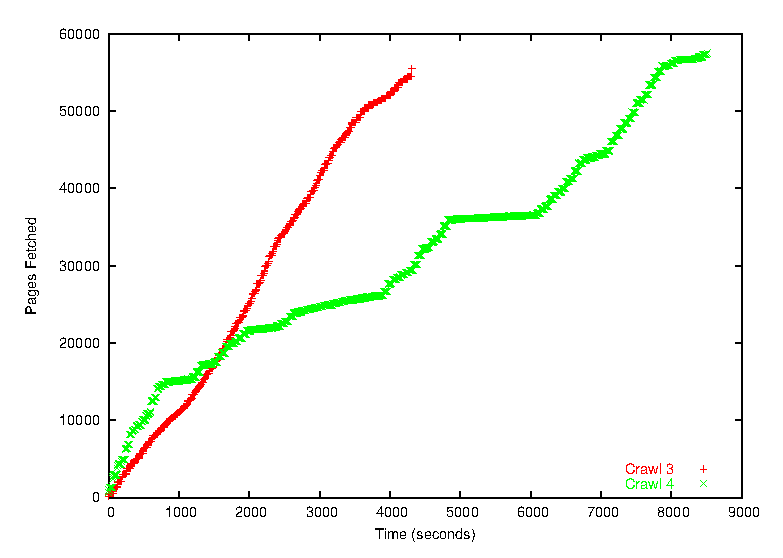
\epsfig{file=./images/crawl4.eps, scale=1.0}
   }
\label{fig-crawl4}
\caption{Crawl 4 (Green) - Seeded with all URLs}
\end{figure}

\begin{figure}[h]
  \centerline{
    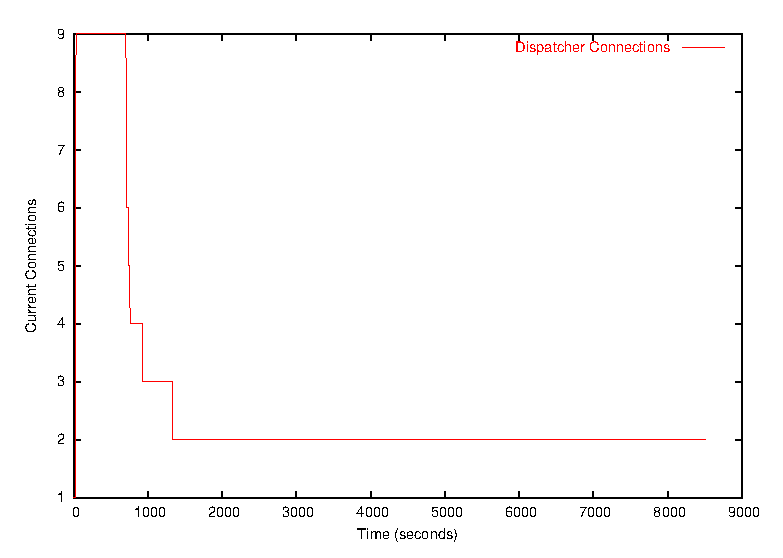
\epsfig{file=./images/crawl4-connections.eps, scale=1.0}
   }
\label{fig-crawl4_connections}
\caption{Crawl 4 - Number of Dispatcher Network Connections}
\end{figure}

\section{PL2 Changes in relation to crawl size}\label{sect-evalpl2}
In Section \ref{sect-terriermatching}, I described the PL2 matching model used by Terrier. He and Ounis describe\cite{ref13} a way of optimising DFR models, such as PL2. This involved tuning the $c$ parameter to acheieve normalisation of term weight to average document length. This is because, in IR, it is current practice to normalise term weight in respect to the length of the document. The c parameter is best normalised for different query sizes.\\
My results are shown in Table \ref{tbl-pl2values} and Figure \ref{fig-pl2}.
\begin{figure}[h]
  \centerline{
    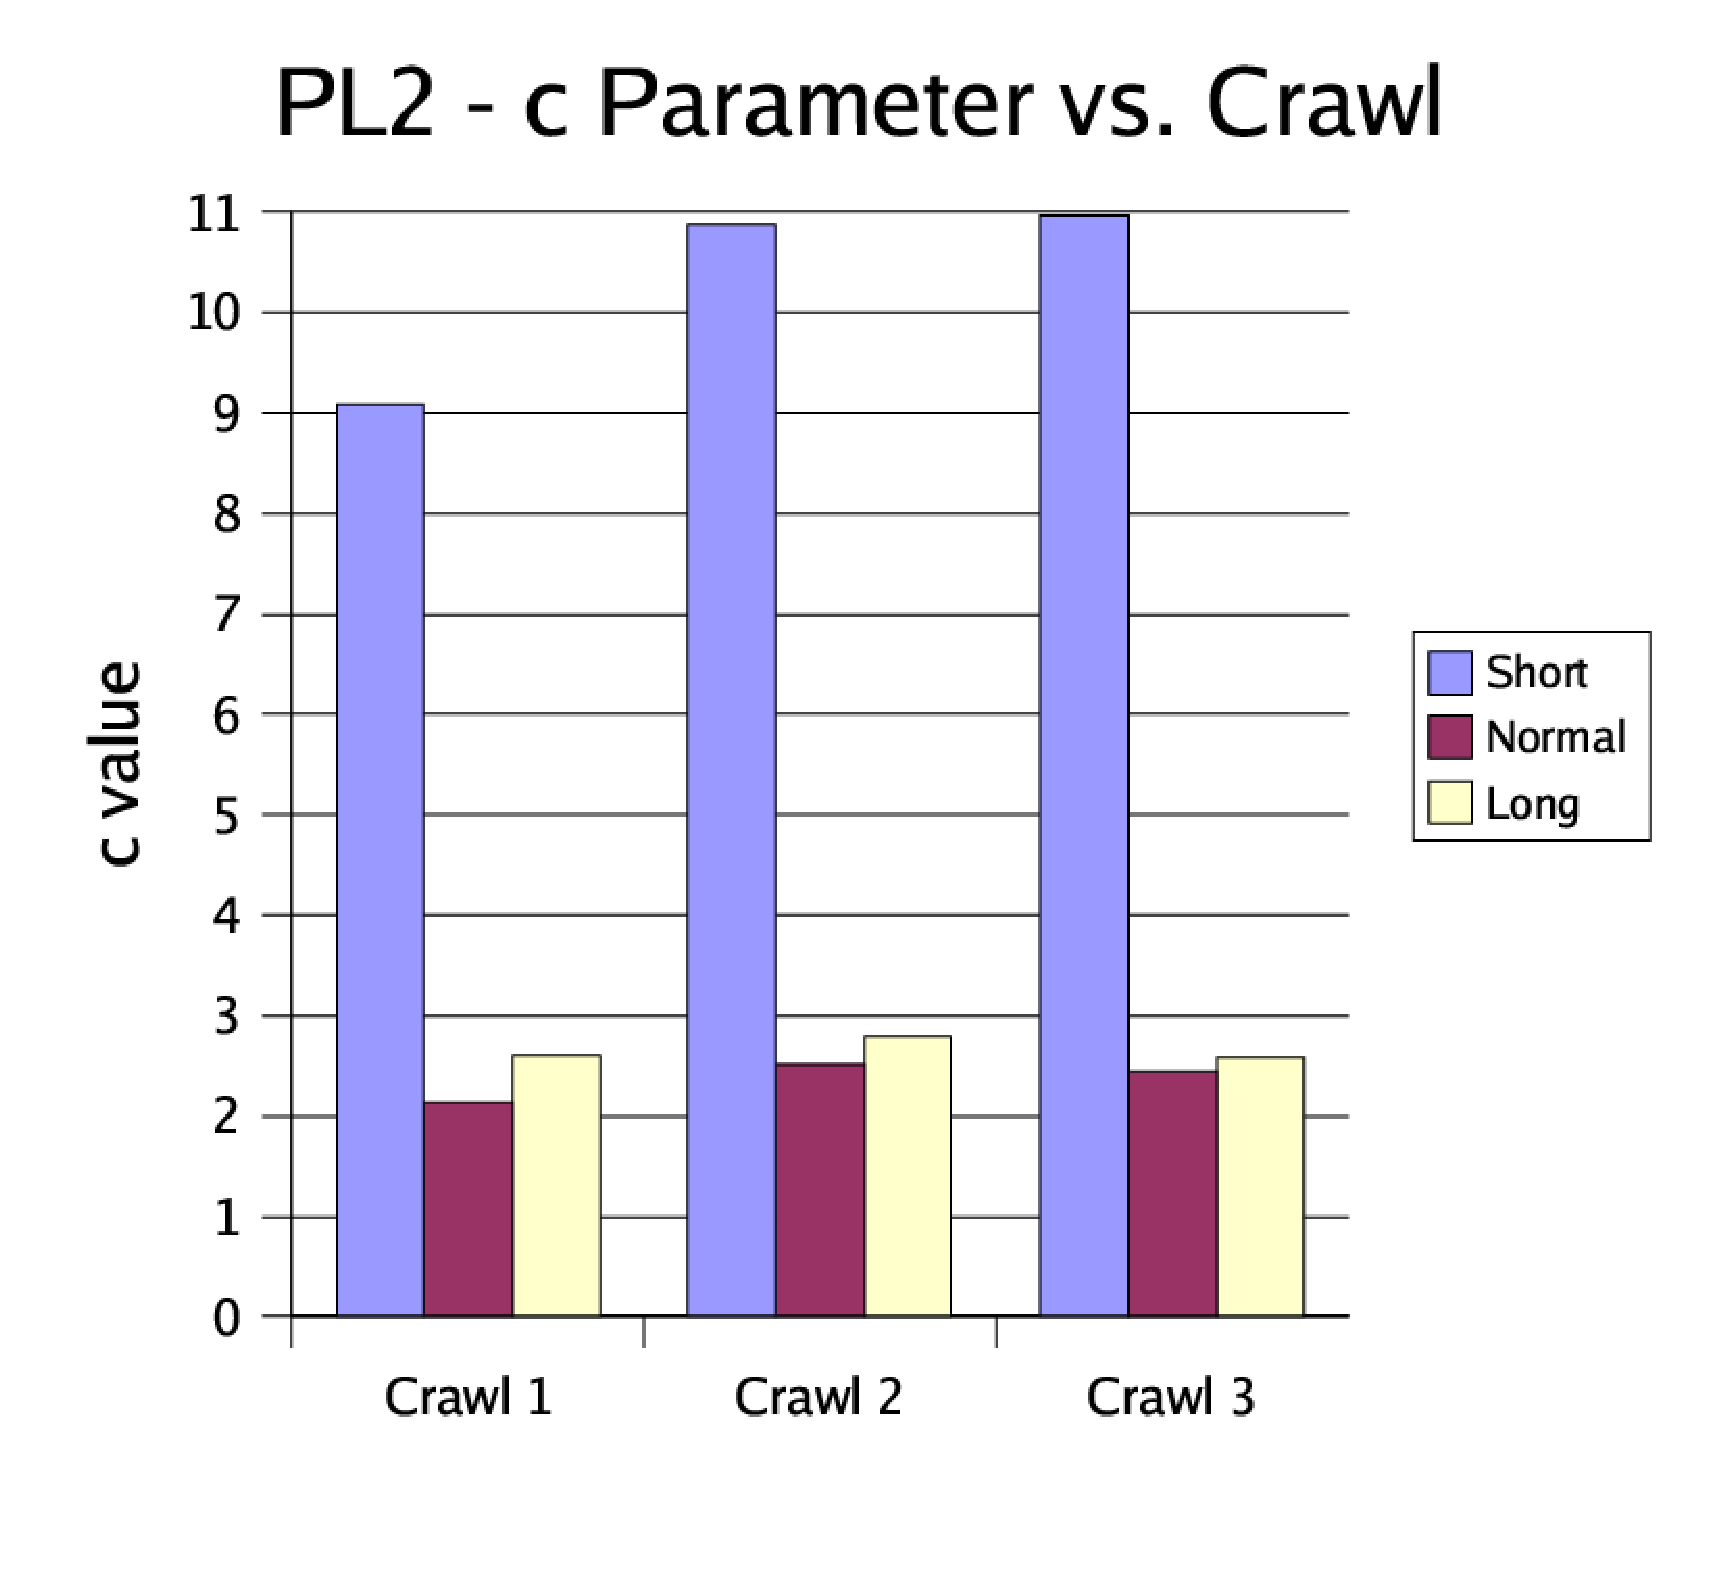
\epsfig{file=./images/graph_pl2c.eps, scale = 0.4}
   }
\label{fig-pl2}
\caption{Affect of increasing crawl size on PL2's $c$ parameter}
\end{figure}
\begin{center}
\begin{table}
\begin{tabular}{|l|l|l|l|}
\hline
\bf{Crawl} & \bf{Query length 1 to 5 words} & \bf{Query length 5 to 12 words} & \bf{Query length more than 12 words} \\
\hline
Crawl 1 & 9.09 & 2.14 & 2.60 \\
\hline
Crawl 2 & 10.88 & 2.51 & 2.79 \\
\hline
Crawl 3 & 10.96 & 2.45 & 2.58 \\
\hline
\end{tabular}
\label{tbl-pl2values}\caption{$c$ Values for different crawls}
\end{table}
\end{center}
This evaluation was performed using three crawls: 1. All externally accessable websites from the Department of Computing Science, Glasgow University; 2. All externally accessable websites of Glasgow University; 3. All externally websites of the Glasgow, Strathclyde, Glasgow Caledonian and Paisley Universities.

\section{Summary}
This evaluation showed the effectiveness of the partitioned mode of the Labrador crawler and of the content filters installed to identify unwanted content during crawls. Test crawls not discussed here show that Labrador can scale to fetching up to millions of pages. I have shown that Discovery period for recrawls could be minimised by seeding the crawl with more URLs, but that care needs to be made in how the seed URLs are partitioned between crawlers. Additionally, the properties of the $c$ parameter of the PL2 DFR matching model over collections has been investigated.


\chapter{Future Work}\label{chp-future}
\section{Refreshing crawls}
According to Kahle(1997), only 40\%\cite{kahle97archiving} of the web pages on the Internet change each month. It clearly follows that recrawling and fetching each page every time a crawl is refreshed is wasteful of resources. Hence many crawlers have implemented recrawling policies that determine which pages will be fetched:
\begin{itemize}
\item{If the page has changed since it was last fetched. This can be achieved using the If-Modified-Since HTTP header, which allows a conditional fetch of the page.}
\item{Based on the importance that the search engine places on the page. This could be based on user feedback about the page (either explicit feedback, or `click-throughs'), or by rating the page's importance using link analysis on the previous crawl.}
\item{Based on the crawler's previous experience about how often the page changes}
\end{itemize}
Obviously, it is desirable that Labrador should be able to save resources by recrawling only the pages that have changed, instead of recrawling the entire target domain when the index needs refreshed. In order to achieve this, Labrador needs to be able to interpret its data files from the previous crawl and use them to obtain the seeding URLs for the next crawl.

\section{URL Ordering}
If the crawler intends to download every page it finds, then any order of URLs suffice. However, if the target crawl domain is larger than the available disk space in which the crawler has to save the crawl\cite{kahle97archiving}, then it is crucial that the more `important' pages are fetched before the lesser ones\cite{ref5}.\\
\ \\
There are many ways to order the queue of URLs to be fetched. Some methods are static, for example based on the order the URLs are discovered - such as Breadth-first (which has been shown to yield quality pages first\cite{ref8}) or Depth-first traversals\footnotemark. Alternative orderings are calculated dynamically, based on a heuristic - examples are:
\begin{itemize}
\item{Using evidence found in the page.}
\item{Back or forward link counts.}
\item{PageRank.}
\end{itemize}

Labrador currently has no provision for dynamically re-ordering its queues, but this would of course be an advantageous development to the system.

\footnotetext{Note that Labrador currently provides both Breadth-first and Depth-first traversal modules}

\section{Topic-focussed Crawler}
On a similar vein, the Information Retrieval Research Group has expressed an interest in Labrador having the capability of being configured as a topic-focussed crawler. Topic-focussed crawlers work similarly to an Internet user browsing web pages of similar topics. The users follow links to pages which they believe to be relevant to them in their topic of interest. Implementing a topic-focussed crawler requires the crawler to be able to rate the relevance of the page to the crawler's topic of interest at crawl time\cite{ref9}. This would be an interesting addition to Labrador's capabilities, allowing futher research to be performed on topic-focussed crawls and Information Retrieval topic-specific collections of data.

\section{Partition Balancing and Migration}
Over the process of crawling a restricted domain crawl, some crawlers may find them unable to keep abreast of the queues for the hosts that have been assigned to them, as they have reached the maximum URLs/second rate they can attain. An indicator of this occuring is when the typical delay between two fetches to one host is greater than the host delay. However, another crawler process may not have enough work to prevent it having to sleep regularly, usually when it is waiting for the host delay to expire on the hosts from which it is currently fetching. In this scenario, it would be more effective if the dispatcher was to recognise this problem and refuse to allocate any more new partitions to the backlogged crawlers, in order to balance the workload evenly between all crawlers. Note that it is not sufficient for the dispatcher to balance the number of partitions assigned to each crawler, because partitions are not necessarily of even sizes. Currently, Labrador will asssign new partitions to the first crawler process that asks for more work. \\
\ \\
Similarly towards the end of a crawl, there are often more crawler processes running than is necesssary. This scenario occurs if more than one crawler is regularly sleeping whilst waiting for Host Delay to expire for its hosts. When this happens, the dispatcher could make the decision to migrate one of the crawlers partitions to the another and shut it down. Note: This would involve the crawler that is to be shutdown having to send its queues back to the dispatcher, to prevent the loss of the queues currently held on that crawler. By consolidating the number of crawler processes, this would free up resources on some crawler machines. However, consolidation should not cause overloading (backlogging) of the crawler machines that remain. Consolidation should only use the excess time each remaining crawler had prior to migration. If a combination of consolidation and balancing is required to achieve the perfect number of crawlers, then the algorithm should have provisions to prevent thrashing, meaning that the some delay should be introduced between a consolidation and balancing operations.

\section{Robustness and Control}
\subsection{Real-time tunability}
Although Labrador comes with a rich configuration file and can highly configured without writing additional code, sometimes it is only once a crawl has started that it becomes apparent that some parameters need adjustment. Examples of this might be:
\begin{itemize}
\item{You wish to reduce the overall network usage. This may be because the crawl is consuming too much of the network's bandwidth, to the detremement of other users on the network.}
\item{A site may have asked to be removed from the current crawl, so has to be blacklisted, with immediate effect.}
\end{itemize}
To perform any of these tasks during a crawl would required configuration changes to be made during the crawl. Unfortunately, Labrador does not support this functionality and the crawl operator has no option but to terminate and restart the crawl to change the configuration. This is because Labrador's communications protocol is based on the crawler processes asking questions of the dispatcher and the dispatcher answering. This leaves no support for pushing information from the dispatcher to each of the clients. I would suggest a UDP server setup on each crawler to allow information to be pushed to crawlers. This could be as simple as just `suggesting' a command that the crawler should execute the next time it calls the dispatcher. Such functionality would allow the dispatcher to inform crawlers of the configuration changes, without having to terminate the crawl.
\subsection{Persistence and Checkpointing}
In a partially-distributed architecture such as Labrador's, the dispatcher is a critical component because the entire crawl will fail should the dispatcher crash. It would be possible for crawlers to continue crawling until the dispatcher returned, however the dispatcher would then have lost its data structures and be unable to continue the crawl.\\
\ \\
The essential functionality required is for the dispatcher to be able to save its data structures to disk occasionally, known as a checkpoint. True ACID properties are not required, it is sufficient that the crawl will repeat the pages between the checkpoint and the crash\cite{ref1}. When the dispatcher is restarted after a crash, it should detect that it had crashed, then restore itself to the state saved at the last checkpoint and recommence the crawl from there.\\
\ \\
Some work has been done towards persistence, however more work needs to be done. For example, currently the dispatcher can restart and restore its data structures. However, in a partitioned crawl, the most valuable data, the URL queues, are maintained at the crawlers. When a crawler fails, the crawl will have lost the queues held at that crawler. Thus a crawl checkpoint should involve the crawlers serializing their URL queues and passing them back to the dispatcher to be checkpointed along with its own data structures.\\
\ \\
Additionally, this would allow bugs in the software of a crawler or dispatcher to be corrected mid-crawl and the crawler restarted, which would be an advantage\cite{ref1}.





\chapter{Conclusion}

\section{Objectives}
Labrador is an advanced scalable and flexible crawler framework, that can be used and extended within the Information Retrieval Research Group to allow for future research, in for example, topic-driven crawling.\\
\ \\
The layered model allows new components to be developed as additional functionality, or more advanced modules dropped in to replace other modules. However, the crawler can be completely re-tasked without changing any code and it provides all the fundamental requirements necessary to do up to medium sized crawls, say to crawl the ac.uk domain.\\
\ \\
However, it is still flexible enough to configure, such that an adminstrator could fine tune its crawling strategy and its rich network API provides monitoring provision for tools such as MRTG.
\section{Summary}
This was a personally interesting project for me to persue, and one that I would like to continue to develop. Crawlers are a very challenging design problem, requiring a program to scale from a few hundred URLs to millions of URLs. The research that has been performed in crawlers is limited and many problems have still to be solved, or optimal methods found.\\
\ \\
With the massive growth the Internet has seen in recent years, the information `somewhere out there' must be made as accessable to users as possible. To this end, it is necessary that techniques are continually evolved to fetch as much important information as possible, indexed in the most efficient way for retrieval purposes, to satisfy the multitude of needs of the population in this `Information Age'.


%\include{chapter_Contributions}

%\include{project_Abbreviation}

\bibliographystyle{biblio}
\bibliography{biblio}
\addcontentsline{toc}{chapter}{Bibliography}

\appendix
\addcontentsline{toc}{chapter}{Appendices}
\chapter{Terrier DTD}\label{terrier_dtd}
\renewcommand{\baselinestretch}{1.0}
\begin{verbatim}
<!DOCTYPE terrier [
<!ELEMENT terrier (results query suggestions?)>

<!ELEMENT query   (#CDATA)>

<!ELEMENT results (result+)>
<!ELEMENT result  (score? url? title? description? results?)>
<!ELEMENT url     (#CDATA)>
<!ELEMENT title   (#CDATA)>
<!ELEMENT description (#CDATA)>
<!ELEMENT score   (#CDATA)>

<!ELEMENT suggestions (suggestion +)>
<!ELEMENT suggestion (score? query)>

<!ATTLIST terrier method CDATA>

<!ATTLIST results count CDATA "0">

<!ATTLIST result number CDATA #REQUIRED>
<!ATTLIST result docid CDATA #REQUIRED>

<!ATTLIST suggestions count CDATA "0">
<!ATTLIST suggestion  number CDATA #REQUIRED>
]>
\end{verbatim}
\renewcommand{\baselinestretch}{1.5}

%\chapter{Frontend Screenshot}\label{appdx-screenshot}
\psfig{figure=images/frontend.eps,height=6in}

\chapter{Protocol Specification}\label{appndx-protocol}
\section{Protocol Syntax}
%\begin{singlespace}  
%\vspace{0cm}
%\renewcommand{\baselinestretch}{1.0}
\begin{center}
%\renewcommand{\baselinestretch}{1.0}

\begin{supertabular}{|l|l|}
\hline
\bf{Client} & \bf{Server} \\
\hline
HELO hostname:pid & \\
Optional header& \\
Optional header& \\
. & 200 Welcome hostname:pid \\
& .\\
\hline
CONF &\\
. & 201 Config follows\\
& Config file contents\\
& Config file contents\\
&.\\
\hline
NEXT (optional no) &\\
. & 202 URLs follow\\
& URL linking\_URL\\
& URL linking\_URL\\
& URL linking\_URL\\
&.\\
&205 No Work \\
\hline
FINISHED url & \\
url found &\\
url found &\\
url found &\\
.&203 Thanks\\
&.\\
\hline
ALLOWED url &\\
.&203 OK to crawl\\
&.\\
&205 Denied by filters\\
&.\\
\hline
ROBOTS hostname &\\
.& 201 Robots.txt follows\\
&Robots.txt file contents\\
&Robots.txt file contents\\
&Robots.txt file contents\\
&.\\
&209 Not yet\\
&.\\
\hline
ROBOTSFILE hostname&\\
Robots.txt file contents&\\
Robots.txt file contents&\\
Robots.txt file contents&\\
.&203 Thanks\\
&.\\
\hline
STATS & \\
statname1: value &\\
statname2: value &\\
statname3: value &\\
statname4: value &\\
.&203 Thanks\\
&.\\
\hline
MONITOR &\\
.&210 Statistics Follow \\
&Stat1Name: Stat1Value \\
&Stat2Name: Stat2Value\\
&.\\
\hline
WORK
&.205 No Work\\
&.\\
&206 Work\\
&no of clients to fork\\
&.\\
\hline
FAILED url&\\
Optional Reason&\\
.&203 Thanks\\
&.\\
\hline
NOOP&\\
.&203 OK\\
&.\\
\hline
QUIT&\\
.&208 Bye!\\
&<DISCONNECT>\\
\hline
CHECKPOINT&\\
.&203 Ok, checkpointed\\
&.\\
\hline
PAUSE&\\
&.203 Ok\\
&.\\
&209 Already paused!\\
&.\\
\hline
START&\\
.&203 Ok\\
&.\\
&209 Not paused!\\
&.\\
\hline
STOP&\\
.&203 Ok\\
&.\\
\hline
FINGERPRINT md5sum&\\
URL&\\
.&201 Seen Already\\
&OtherURL\\
&.\\
&209 First Time Seen\\
&.\\
\hline
CHECKPOINT&\\
.&203 Ok\\
&.\\
\end{supertabular}
%\renewcommand{\baselinestretch}{1.5}
\end{center}
%\renewcommand{\baselinestretch}{1.5}
%\end{singlespace}

\section{Verb Descriptions}
\subsection{HELO}
I am a client, ready to do work. Here is my unique crawler name

\subsection{CONF}
I'd like to know what my configuration should be. Can you please tell me it?

\subsection{NEXT}
Could I have some URLs to work on please? If followed by an integer, this is the number of URLs I'd like to work on, if possible.

\subsection{FINISHED}
I've finished parsing this URL. Here are the links it contained - you should add these to your queue for filtering and crawling

\subsection{ROBOTS}
Do you have the robots.txt file for hostname?

\subsection{ROBOTSFILE}
Here is the contents of the robots.txt file for hostname that I fetched. Please save it in your cache.

\subsection{STATS}
Here are my stats, add these to your totals.

\subsection{MONITOR}
Please give me all your available stats.

\subsection{WORK}
Is there any work available yet? I'd like to fork some clients to do some work for you.

\subsection{NOOP}
No operation - just checking the connection is OK. Meaningless verb.

\subsection{ALLOWED}
Can you check that this URL is allowed by the URL filters?

\subsection{FINGERPRINT}
Here is the fingerprint of this URL. Can you check if you've seen it before and if so where?

\subsection{CHECKPOINT}
Please checkpoint your data structures to disk now.

\subsection{QUIT}
This process is shutting down (or at least disconnecting). Please disconnect me.
\subsection{PAUSE}
Temporarily pause the crawl. May not have effect in partitioned crawls. Crawlers may timeout during an extended pause.
\subsection{START}
End a pause started using the PAUSE.
\subsection{STOP}
Terminate the crawl. May take some time to have effect in partitioned crawls.

\section{Notes}
Only HELO, NOOP and QUIT are permitted if a client hasn't logged on yet. HELO is called to logon. Additional permissions are viewable in Table \ref{tbl-commands}.

\section{Return Messages}
Return messages by the dispatcher are of the form:
\begin{verbatim}
StatusNumber[space]Friendly Error Message
Optional parameters
.
\end{verbatim}
Generally speaking 2xx should be success error messages, and 3xx for messages.\\
\begin{center}
\begin{tabular}{|l|}
\hline
\bf{Generic (Error) Messages}\\
\hline
300 Client Error (produced in software by the client)\\
301 Unknown Command\\
302 Unimplemented Command\\
303 Permission Denied. (Client has insufficient privileges to execute command)\\
304 Bad Syntax\\
\hline
\end{tabular}
\end{center}

\chapter{Sample Configuration File}\label{appndx-config}
\renewcommand{\baselinestretch}{1.0}
\begin{verbatim}
#This is the global configuration file for Labrador Web Crawler
#for crawling all externally available hosts in gla.ac.uk

#if omitted, defaults to folder above binary (../)
Base /local/terrier_tmp/macdonch/labrador/

#what port to run the dispatcher on, default 2680
DispatcherPort 2680

#number of subcrawlers to fork on each machine
ForksPerCrawler 4

#the MD5 of the password that must be send before admin
#privilege commands are allowed to be executed
AdminPassword LczRqz4DmQrqdzWYMchcog

#minumum number of seconds between each request to a
#given hostname
HostDelay 3

ObtainURLs data/rootsets/rootset_gla1.txt

#days until a robots.txt file expires
RobotsTxtExpiry 25

#File to log all dispatcher communications to 
#DispatcherCommsLog data/comms.txt

#where to put a robots.txt cache directory
#RobotsTxtCache data/robots.txt/

#URL allocation - eg DFS, BFS etc
#implementation detail - BFS adds to end of main queue,
#DFS adds to start
URLAlloc BFS

#takes from the head of the main queue, and allocates
#each URL to a crawler host
#this only encapsulates data manipulation, not storage

#we're using a partitioned crawl
CrawlerAlloc Partitioned

#URLFilter ModuleHandler (params)
URLFilter Regexp URL =~ ^http(?:s?)://(?:[A-Za-z0-9\-.]+)\.gla\.ac\.uk
URLFilter File Whitelist Host data/whitelists/hosts_gla.txt
URLFilter File Blacklist Host data/blacklists/hosts_gla.txt
URLFilter File Blacklist Extension data/blacklists/extensions_gla.txt
URLFilter File Blacklist URL data/blacklists/urls_gla.txt
#dont follow links into any calendar type web pages
URLFilter Regexp Querystring !~ calendar

#next two are fairly self-explanatory - basically crawler trap protection
URLFilter URLDepth 15 
URLFilter Length 1024


#DNS prelookup - disabled for small crawls
#we want DNSlookup to be last
#URLFilter DNSLookup 
#passes to another process across a pipe or a 
#socket to perform async lookups, ignores result


#limit request to same filename with different querystring
#currently only enabled with Manager Partitioned
MaxFilenameRequests 200

DataPersistence Hash GDBM_File
DataPersistence Array Tie::File
PersistenceCheckpointEvery 1200

#end the crawl after successfully downloading MaxCrawlURLs urls
#defaults to 0, which means unlimited
MaxCrawlURLs 0


#FROM HERE DOWN IS FOR THE SUBCRAWLERS
#run a partitioned crawl
Manager Partitioned
PartitionedAlloc Delay
Partition SeenHost

#Proxy server details
#SpiderProxy http://wwwcache.dcs.gla.ac.uk:8080
#SpiderProxyUsername
#SpiderProxyPassword

#required - the HTTP Header name field each spider should give
SpiderName Labrador

#Required
SpiderVersion 0.2

#required - the HTTP Header email field each spider should give
SpiderEmail macdonch@dcs.gla.ac.uk

#content filters
#NB: these must contains ContentTypes and MetaRobots (in that
#order) unless you are absolutely positive you know what you
#are doing
ContentFilter ContentTypes
ContentFilter MetaRobots
ContentFilter Fingerprint #prevents duplicate documents being indexed or followed
ContentFilter Binary #ignore any files containing the null character

MD5Fingerprints 1

#LWP activity timeout - try to keep a decent url rate up!
Timeout 5

#limit the size of each crawler before it retires
#MaxCrawlerRequests 400

#List of HTML tags which contain links to follow
#other possible options are img:
FollowTagLinks a area meta link

#content types to index
IndexContentTypeWhitelist text/html text/plain application/xhtml+xml \
 application/postscript application/pdf text/xml 

#content types to process for links
FollowContentTypeWhitelist text/html application/xhtml+xml text/xml

#ContentHandler HandlerModule (params?)
ContentHandler PreTerrier /local/terrier_tmp/macdonch/crawls/crawl_gla/saved/


#SpiderSyncStats time in seconds to tell the dispatcher your stats
#default 3600 (1 hour)
SpiderSyncStats 60

#Where to save access logs to
SpiderAccessLog /local/terrier_tmp/macdonch/crawls/crawl_gla/logs/access-%H-%P.log

#Format of log files
# %a - Remote IP address
# %A - Remote hostname
# %d - sprintf standard date format
# %f - Filename
# %p - Remote port
# %T - Time taken to make request
# %t - Current epoch time
# %m - Request method
# %q - Querystring
# %U - entire URL requested
# %u - URI of request
# %s - HTTP status code
# %S - Protocol scheme (eg http, https)
# %r - Referring URL
# %c - Size of content downloaded uncompressed (excluding headers)
# %C - Size of content downloaded compressed (excluding headers)
# %P - PID of requesting crawler
# %H - the hostname of the requesting crawler
SpiderAccessLogFormat "%t %s %c %A %u %U %b %B %T"
\end{verbatim}
\renewcommand{\baselinestretch}{1.0}


\end{document}
